\documentclass[mat1, tisk]{fmfdelo}
% \documentclass[fin1, tisk]{fmfdelo}
% Če pobrišete možnost tisk, bodo povezave obarvane,
% na začetku pa ne bo praznih strani po naslovu, …

%%%%%%%%%%%%%%%%%%%%%%%%%%%%%%%%%%%%%%%%%%%%%%%%%%%%%%%%%%%%%%%%%%%%%%%%%%%%%%%
% METAPODATKI
%%%%%%%%%%%%%%%%%%%%%%%%%%%%%%%%%%%%%%%%%%%%%%%%%%%%%%%%%%%%%%%%%%%%%%%%%%%%%%%

% - vaše ime
\avtor{Jaša Knap}

% - naslov dela v slovenščini
\naslov{Kratki zakoni v grupah}

% - naslov dela v angleščini
\title{Short Group Laws}

% - ime mentorja/mentorice s polnim nazivom:
%   - doc.~dr.~Ime Priimek
%   - izr.~prof.~dr.~Ime Priimek
%   - prof.~dr.~Ime Priimek
%   za druge variante uporabite ustrezne ukaze
\mentor{doc.~dr.~Urban Jezernik}
% \somentor{...}
% \mentorica{...}
% \somentorica{...}
% \mentorja{...}{...}
% \somentorja{...}{...}
% \mentorici{...}{...}
% \somentorici{...}{...}

% - leto diplome
\letnica{2024} 

% - povzetek v slovenščini
%   V povzetku na kratko opišite vsebinske rezultate dela. Sem ne sodi razlaga
%   organizacije dela, torej v katerem razdelku je kaj, pač pa le opis vsebine.

\povzetek{Bistvo diplomske naloge je predstaviti različne konstrukcije kratkih netrvialnih zakonov v grupah. Pri tem obravnavamo naravne družine grup, ki se pri tem pojavijo, kot so na primer nilpotentne, rešljive, enostavne in simetrične. Na koncu predstavimo, kako se iskanja zakonov lotimo z uporabo računalnika.}

% - povzetek v angleščini

% \abstract{The main purpose of this thesis is to present several different constructions of short group laws. In order to do so, we observe the properties of nilpotent, solvable, simple and symmetric groups. The thesis is concluded by demonstrating how computers can be used for finding group laws.}
\abstract{The purpose of this thesis is to present various constructions of short group laws. In order to do so, we examine the properties of nilpotent, solvable, simple, and symmetric groups. The thesis is concluded by illustrating how computational methods can be used to discover group laws.}

% - klasifikacijske oznake, ločene z vejicami
%   Oznake, ki opisujejo področje dela, so dostopne na strani https://www.ams.org/msc/
\klasifikacija{20F10, 20F14, 20D15, 20B30}

% - ključne besede, ki nastopajo v delu, ločene s \sep
\kljucnebesede{zakoni v grupah \sep proste grupe \sep nilpotentne grupe \sep rešljive grupe \sep enostavne grupe \sep simetrične grupe \sep naključni sprehodi po grafih \sep Cayleyjevi grafi \sep računalniško iskanje zakonov}

% - angleški prevod ključnih besed
\keywords{group laws \sep free groups \sep nilpotent groups \sep solvable groups \sep simple groups \sep symmetric groups \sep random walks on graphs \sep Cayley graphs \sep computer-aided } % angleški prevod ključnih besed 

% - angleško-slovenski slovar strokovnih izrazov

\slovar{
% \geslo{angleški izraz}{slovenski izraz}
% ...
\geslo{group law/identity}{zakon v grupi}
\geslo{nilpotent group}{nilpotentna grupa}
\geslo{solvable group}{rešljiva grupa}
\geslo{simple group}{rešljiva grupa}
\geslo{non-trivial power}{periodični element}
\geslo{symmetric group}{simetrična grupa}
\geslo{lower central series}{spodnja centralna vrsta}
\geslo{derived series}{izpeljana vrsta}
\geslo{(lazy) random walk}{(leni) naključni sprehod}
}

% - ime datoteke z viri (vključno s končnico .bib), če uporabljate BibTeX
\literatura{literatura.bib}

%%%%%%%%%%%%%%%%%%%%%%%%%%%%%%%%%%%%%%%%%%%%%%%%%%%%%%%%%%%%%%%%%%%%%%%%%%%%%%%
% DODATNE DEFINICIJE
%%%%%%%%%%%%%%%%%%%%%%%%%%%%%%%%%%%%%%%%%%%%%%%%%%%%%%%%%%%%%%%%%%%%%%%%%%%%%%%

% naložite dodatne pakete, ki jih potrebujete
% \usepackage{...}

\usepackage{tikz-cd}
\usepackage{cancel}

% \usepackage{quiver}
% \usepackage{listings}

% deklarirajte vse matematične operatorje, da jih bo LaTeX pravilno stavil
% \DeclareMathOperator{\...}{...}

\newcommand{\bigslant}[2]{{\raisebox{.2em}{$#1$}\left/\raisebox{-.2em}{$#2$}\right.}}

\numberwithin{equation}{section}  % števec za enačbe zgleda kot (2.7) in se resetira v vsakem razdelku
\newenvironment{skica}[1][Skica dokaza]{\begin{proof}[#1]}{\end{proof}}

\newcommand{\propernormalsubgroup}{%
  \mathrel{\ooalign{$\lneq$\cr\raise.22ex\hbox{$\lhd$}\cr}}}
% vstavite svoje definicije ...
% \newcommand{\...}{...}

%%%%%%%%%%%%%%%%%%%%%%%%%%%%%%%%%%%%%%%%%%%%%%%%%%%%%%%%%%%%%%%%%%%%%%%%%%%%%%%
% ZAČETEK VSEBINE
%%%%%%%%%%%%%%%%%%%%%%%%%%%%%%%%%%%%%%%%%%%%%%%%%%%%%%%%%%%%%%%%%%%%%%%%%%%%%%%

\begin{document}

 
\section{Uvod}
Začnimo z inuitivno definicijo zakona v grupi, ki jo bomo v nadaljevanju natančneje formulirali s pomočjo prostih grup.
Abstraktni produkt elementov $a_1, \ldots , a_k$ ter njihovih inverzov $a_1^{-1}, \ldots , a_k^{-1}$ je \emph{$k$-črkovni zakon v grupi $G$}, če ima lastnost, da za vsako zamenjavo $a_1, \ldots, a_k$ s konkretnimi
elementi $g_1, \ldots, g_k \in G$ dobimo rezultat $1_G\in G$. Zakonu $1$ pravimo \emph{trivialni zakon}, ki v kontekstu raziskovanja zakonov ni posebej zanimiv.

Najosnovnejši primer netrivialnega dvočrkovnega zakona se pojavi pri Abelovih grupah. Grupa $G$ je namreč Abelova natanko tedaj, ko za vsaka elementa $g, h \in  G$ velja $gh = hg$, kar je ekvivalentno
zahtevi \begin{equation*}
ghg^{-1}h^{-1} = [g,h] = 1_G.
\end{equation*}
Grupa $G$ je torej Abelova natanko tedaj, ko je štiričrkovna beseda $aba^{-1}b^{-1}$ v njej zakon. 

Nadvse pomembno je vprašanje, ali vsaka grupa premore netrivialni zakon. Odgovor nanj je v splošnem negativen, kar bomo videli v nadaljevanju kot posledico trditve \ref{trd_dolzina_zakonov_za_psl2p}. 
Očitna posledica Lagrangeevega izreka pa je, da vsaka končna grupa $G$ premore
netrivialni zakon $a^{\lvert G \rvert }$, saj za vsak element $g \in G$ velja  
\begin{equation*}
g^{\lvert G \rvert } = 1_G.
\end{equation*}  

To dejstvo si natančneje oglejmo na primeru simetrične grupe $\text{Sym}(n)$. Zanjo po Lagrangeevem izreku velja enočrkovni zakon $a^{n !}$, katerega dolžina znaša $n!$, kar je po Stirlingovi formuli približno
\begin{equation*}
n! \sim \sqrt{2 \pi n} \left( \frac{n}{e} \right)^{n}.
\end{equation*}  
Asimptotsko gledano je to zelo dolg zakon, veliko krajši je na primer že zakon oblike $a^{\exp(\text{Sym}(n))}$, kjer smo označili $\exp(\text{Sym}(n)) = \text{lcm}(1, \ldots, n)$. Zanj s pomočjo praštevilskega izreka \ref{lem_gostota_prastevil} 
% TODO tule moraš popraviti to referenco!! 
% TODO dokaži oceno !!
dobimo asimptotsko oceno \begin{equation*}
\text{lcm}(1, \ldots ,n) \sim e^{n}.
\end{equation*}  
Trenutno najboljša ocena za dolžine kratkih zakonov v simetričnih grupah izhaja iz članka \cite{Kozma_Thom_2016} in bo predstavljena v razdelku \ref{sec_simetricne_grupe}.

Na tej točki se naravno pojavi nekaj vprašanj: kako dolgi so najkrajši netrivialni zakoni za določeno grupo oziroma družino grup? Ali lahko ocenimo
asimtotsko rast dolžine najkrajših netrivialnih zakonov v družinah grup, recimo za družino $\text{Sym}(n)$? Kaj pa za vse grupe moči $n$ ali manj? 
Katere družine grup se še posebej naravno pojavljajo pri takšnem raziskovanju?
Prav ta vprašanja bodo bistvo diplomske naloge, v kateri bom predstavil dosedanje
rezultate ter različne pristope, ki so jih ubrali raziskovalci. Na koncu bom predstavil,
kako lahko z uporabo računalnika dobimo vpogled v delež zakonov med vsemi besedami.

Zgodovinsko gledano so vprašanja v povezavi z asimptotskimi lastnostmi zakonov razmeroma sodobna. V splošnem pa obravnavanje lastnosti zakonov v nekem smislu sega že do Abela in Galoisa, 
saj lahko tako Abelove kot rešljive grupe zelo naravno karakteriziramo s pomočjo zakonov. Zakoni so pomembni tudi za obravnavo klasičnih Bursidovih problemov,
ki matematikom burijo domišljijo že od začetka 20.~stoletja. Ti problemi sprašujejo po končnosti specifičnih kvocientov prostih grup, kar bo nekoliko podrobneje razloženo v
razdelku \ref{sec_racunalnisko_iskanje}. 

% Zakone lahko recimo uporabljamo za prezentacijo grup, morda najbolj znani primer predstavljajo diedrske grupe \begin{equation*}
%     D_{2n} = \langle r, Z  \vert  r^{n} = Z^{2} = 1, (rZ)^2 = 1 \rangle.  
%     \end{equation*}  
%     Diedrska grupa je enolično določena s tremi enočrkovnimi zakoni, ki jim morata ustrezati generatorja $r$ in $Z$ ($a^{n}$ in $a^{2}$) oziroma njun produkt $rZ$ ($a^{2}$).

\section{Osnovni pojmi za obravnavo zakonov}

Za natančno formulacijo in razumevanje zakonov moramo uvesti pojem proste grupe.

\subsection{Proste grupe}

Naslednjo definicijo proste grupe najdemo v članku \cite{Pogacnik_2024}.

\begin{definicija}
\label{def_prosta_grupa}
Grupa $F$ je \emph{prosta} nad neprazno množico $S$, če za vsako preslikavo $\iota : S \to F$ in vsako grupo $G$ in vsako preslikavo $\iota: X \to  G$ obstaja natanko en homomorfizem $\tilde{\varphi} \in \operatorname{Hom}(F, G)$,
da velja $\tilde{\varphi} \circ \iota = \varphi$. Z drugimi besedami, spodnji diagram komutira. Tej lastnosti pravimo \emph{univerzalna lastnost prostih grup}.
 % TODO dodaj ta diagram
\end{definicija}

% https://q.uiver.app/#q=WzAsMyxbMCwwLCJYIl0sWzIsMCwiRyJdLFswLDIsIkYiXSxbMCwxLCJcXHZhcnBoaSJdLFswLDIsIlxcaW90YSIsMl0sWzIsMSwiXFx0aWxkZXtcXHZhcnBoaX0iLDIseyJzdHlsZSI6eyJib2R5Ijp7Im5hbWUiOiJkYXNoZWQifX19XV0=
% \begin{tikzcd}
% 	X & G \\
% 	\\
% 	F
% 	\arrow["\varphi", from=1-1, to=1-3]
% 	\arrow["\iota"', from=1-1, to=3-1]
% 	\arrow["{\tilde{\varphi}}"', dashed, from=3-1, to=1-3]
% \end{tikzcd}

\begin{trditev}
\label{trd_enolicnost_prostih_grup}
 Naj bo $S$ neprazna množica. Potem do izomorfizma natančno obstaja največ ena prosta grupa nad množico $S$.
\end{trditev}
\begin{dokaz}
Dokaz trditve je vzet iz \cite[str.~4]{Pogacnik_2024}.
Naj bosta $F$ in $F'$ prosti grupi nad množico $S$. Označimo z $i$ in $j$ inkluziji $i : S \to F$ in $j : F'$, ki jima po definiciji \ref{def_prosta_grupa} pripadata. Po univerzalni lastnosti prostih grup lahko inkluziji
razširimo do homomorfizmov $\varphi_i : F' \to F$ in $\varphi_j : F \to F'$. (TODO vstavi komutativni diagram)
Kompozitum $\varphi_i \circ \varphi_j : F \to F$ je na množici $S$ identiteta. Ker sta tako $\varphi_i \circ \varphi_j$ kot $\text{id}_F$ razširitvi inkluzije $i$,
mora po enoličnosti razširitev veljati $\varphi_i \circ \varphi_j = \text{id}_F$. Simetrično pokažemo še $\varphi_j \circ \varphi_i  = \text{id}_{F'}$, torej sta grupi $F$ in $F'$ izomorfni.
\end{dokaz}

Zaradi te trditve je $F(S)$ upravičena oznaka za prosto grupo nad množico $S$. Še več, grupi $F(S)$ in $F(T)$ sta si izomorfni kot grupi natanko tedaj, ko sta si $S$ in $T$ izomorfni kot množici.
Zato bomo v primeru, ko je $S$ končna množica moči $k$, namesto $F(S)$ pisali $F_k$.

Naj bo sedaj $S$ poljubna neprazna množica. Definiramo grupo okrajšanih besed nad množico $S$ kot \begin{equation*}
    S^* := \{ s_1 s_2 \cdots s_n  \vert n \in \mathbb{N}, \forall i = 1, \ldots, n.\,  s_i \in S \cup S^{-1} , \forall i = 1 , \ldots n-1 .\, s_i \neq s_{i + 1}^{-1} \}.
\end{equation*}
Operacija nad njej je stikanje besed, ki jim nato še okrajšamo sosednje inverze. Ta operacija je dobro definirana, grupa $S^*$ pa prosta nad množico $S$. 
Ti dejstvi sta natančno dokazani v viru (\cite[str.~4, tridtev 1.9]{Lyndon_Schupp_2015}). Po trditvi \ref{trd_enolicnost_prostih_grup} sledi $S^* \cong F(S)$,
zato si lahko elemente prostih grup predstavljamo kot okrajšane besede. Z upoštevanjem tega dejstva lahko elementom proste grupe $F(S)$ definiramo dolžino.

\begin{definicija}
\label{def_dolzina_besede}
Naj bo beseda $w \in  F(S)$ oblike $w = s_1 \cdots s_n$. Potem število $l(w) := n$ imenujemo \emph{dolžina besede $w$}.
\end{definicija}
\begin{opomba}\label{opm_trikotniska_neenakost}
    Po definiciji množenja besed v prostih grupah je očitno, da za vsaki besedi $w_1 , w_2$ velja trikotniška neenakost $l(w_1 w_2) \le l(w_1) l(w_2)$.
\end{opomba}

Pri konstrukciji zakonov stalno uporabljamo naslednjo na videz očitno trditev, ki jo vendarle moramo dokazati. 

\begin{trditev}\label{trd_prosta_grupa_je_torzijsko_prosta}
    Proste grupe so \emph{torzijsko proste}. Z drugimi besedami, vsi elementi razen enote so neskončnega reda. 
\end{trditev}
\begin{dokaz}
    Naj bo $F(S)$ prosta grupa nad neprazno množico $S$. Recimo, da obstaja beseda $w \in F(S)$ končnega reda oblike $w = a_1 a_2 \ldots a_n$ za paroma neinverzne $a_1, \ldots , a_n \in S$. Naj bo preslikava $j : S \to (\mathbb{Z}, +)$, ki vse elemente $a_i$ slika v pozitivna števila. Po univerzalni lastnosti prostih grup jo lahko razširimo do homomorfizma $\varphi_j \in \operatorname{Hom}(F(S), \mathbb{Z})$. 
    Ker je $\varphi_j$ homomorfizem, bo $\varphi(w) = \sum_{i = 1}^{n} \varphi(a_i) > 0$. To je prosislovno, saj bi moral red elementa $\varphi(w)$ deliti red besede $w$,
    grupa $(\mathbb{Z}, +)$ pa je torzijsko prosta, zato je element $\varphi_j(w)$ v njej neskončnega reda.
\end{dokaz}


Brez dokaza bomo privzeli Nielsen--Schreierjev izrek, ki je klasični rezultat v teoriji prosti grup. Potrebovali ga bomo za dokaz komutatorske leme,
še bolj izrazito pa pri obravnavi zakonov z računalnikom v razdelku \ref{sec_racunalnisko_iskanje}. 

\begin{izrek}[Nielsen--Schreierjev izrek]
\label{izr_nielsen_schreier}
 Vsaka podgrupa proste grupe je prosta.
\end{izrek}

Bralec lahko dokaz najde v \cite[str.~5--8]{Lyndon_Schupp_2015}.

\subsection{Definicija in osnovne lastnosti zakonov}\label{sec_osnovne_lastnosti_zakonov}

Za začetek uvedimo blago zlorabo notacije. Naj bo podana prosta grupa $F_k = \langle a_1, \ldots, a_k \rangle$ in naj bo $w$ beseda v njej.
Naj bo $G$ grupa in naj bodo $g_1, \ldots, g_k \in G$. Potem definiramo \begin{equation*}
    w(g_1, \ldots, g_k) := \varphi(w),
\end{equation*}
kjer je $\varphi \in \operatorname{Hom}(F_k, G)$ po univerzalni lastnosti induciran s slikami $a_i \mapsto g_i$ za $i = 1, \ldots, k$.
To je formalna definicja intuitivne ideje \glqq vstavljanja konkretnih elementov grupe v abstraktne elemente\grqq iz uvodnega poglavja. Z njeno pomočjo definiramo zakone.

\begin{definicija}\label{def_zakon_formalna}
    Beseda $w \in F_k$ je \emph{$k$-črkovni zakon v grupi $G$}, če za vse $k$-terice elementov $g_1, \ldots, g_k \in G$ velja $w(g_1, \ldots, g_k) = 1_G$.
    Za vsako podgrupo $H \le G$ pravimo tudi, da je $w \in F_k$ \emph{$k$-črkovni zakon v podgrupi $H$}, če za vse $k$-terice elementov $h_1, \ldots, h_k \in H$ velja $w(h_1, \ldots, h_k) = 1_G$.
\end{definicija}

Ta definicija nam omogoča vpogled v strukturo zakonov. Naj \emph{$K(G, k) \subseteq F_k$ označuje množico $k$-črkovnih zakonov v grupi $G$}. Potem v luči prejšnje definicije velja
\begin{equation*}
K(G, k)  = \bigcap_{\varphi \in \operatorname{Hom}(F_k, G)} \ker(\varphi).   
\end{equation*}  
Ta množica je končni presek edink v $G$ in posledično tudi sama edinka. Še več, je karakteristična, saj za vsak avtomorfizem $\alpha \in \operatorname{Aut}(F_2)$ velja
\begin{equation*}
    K(G, k)  = \bigcap_{\varphi \in \operatorname{Hom}(F_k, G)} \ker(\varphi) = \bigcap_{\varphi \in \operatorname{Hom}(F_k, G)} \ker(\varphi \circ \alpha). 
\end{equation*}  
To je preprosta posledica dejstva, da $\varphi$ preteče grupo $\operatorname{Hom}(F_k, G)$ natanko tedaj, ko jo preteče $\varphi \circ \alpha$.     

\begin{lema}\label{lem_koncni_indeks_koncnega_preseka}
Naj bo $G$ grupa ter $H_1, \ldots, H_n$ njene podgrupe končnega indeksa, torej $[G: H_i] < \infty$ za $i = 1, \ldots, n$. Potem je tudi $\bigcap_{i = 1}^{n} H_i$ podgrupa končnega indeksa v $G$ in velja
\begin{equation*}
\left[ G: \bigcap_{i = 1}^{n} H_i \right]  \le \prod_{i=1}^{n} [G: H_i].  
\end{equation*} 
\end{lema}

\begin{dokaz}
Dovolj je dokazati trditev za $n = 2$, za višje vrednosti sledi z indukcijo. Naj bosta $H_1, H_2 \le G$ podgrupi končnega indeksa, označimo $S: = H_1 \cap H_2$, ki je podgrupa v $G$. Naj bosta $A_1$ in $A_2$ množici odsekov podgrup $H_1$ in $H_2$ v $G$ ter naj bo $A$ množica odsekov podgrupe $S$ v $G$.
 Definiramo preslikavo $f : A \to  A_1 \times A_2$ s predpisom $f(g S ) = (g H_1, g H_2)$. Desna smer sklepa \begin{equation*}
 g S = h S \iff gh^{-1} \in H_1, \, gh^{-1} \in H_2  \iff g H_1 = h H_1, \, g H_2 = h H_2
\end{equation*}  
nam podaja dobro definiranost, leva pa injektivnost preslikave $f$, ki nam podaja oceno $\lvert A \rvert \le  \lvert A_1 \rvert \lvert A_2 \rvert $.    
\end{dokaz}
Z uporabo te leme direktno sledi, da je v primeru končnosti grupe $G$ grupa $K(G, k)$ podgrupa končnega indeksa največ $\lvert G \rvert^{ \lvert G \rvert^k}$ v $F_k$. 
Za vsak homomorfizem $\varphi \in \operatorname{Hom}(F_k, G)$ namreč po prvem izreku o izomorfizmu velja \begin{equation*}
    \lvert F_k / \ker \varphi \rvert = \lvert \operatorname{im} \varphi \rvert \le \lvert G \rvert. 
\end{equation*}
To dejstvo bo še posebej pobmembno pri iskanju zakonov z računalnikom.


\begin{definicija}
\label{def_cayleyev_graf}
Naj bo $G$ grupa in $S \subseteq G$ njena \emph{simetrična} podmnožica. To pomeni, da velja $S = S^{-1} := \{ s^{-1}  \vert s \in S  \}$. Potem $\operatorname{Cay}(G, S)$ označuje graf z vozlišči $V = G$ in povezavami
$E = \left\{ (p, q) \middle|\, p^{-1}q \in  S \right\}$. Imenujemo ga \emph{Cayleyjev graf grupe $G$, generiran z množico $S$}.  
\end{definicija}

\begin{opomba}
Pogoj simetričnosti $S = S^{-1}$ nam pove, da je $\operatorname{Cay}(G, S)$ pravi graf in ne zgolj usmerjen. Imamo namreč \begin{equation*}
(p,q) \in  E \iff p^{-1}q \in S \iff q^{-1}p \in S \iff (q,p) \in  E.
\end{equation*}  
\end{opomba}

Preden si ogledamo dva primera, dokažimo nasledjo preprosto, a pomembno trditev.

\begin{trditev}\label{trd_lastnosti_cayleyjevega_grafa}
    Naj bo $S$ končna grupa moči $k$. Cayleyjev graf $\text{Cay}(G, S)$ je $\lvert S \rvert$-regularen, povezan graf.
\end{trditev}
\begin{dokaz}
    Naj bo $g \in G$ vozlišče Cayleyjevega grafa $\text{Cay}(G, S)$. Potem je $g$ povezano z enoto $1_G$, saj je $\langle S \rangle = G$, torej lahko zapišemo
    $g = s_1 s_2 \cdots s_n$ za neke elemente $s_i \in S$. Ta produkt določa povezavo v Cayleyjevem grafu. Ker je vsako vozlišče povezano z enoto $1_G$, je graf povezan. Iz $g s_i = g s_j$ sledi $s_i = s_j$, zato iz vsakega vozlišča vodi natanko $\lvert S \rvert$ različnih povezav.
\end{dokaz}

\begin{primer}
Na spodnjih slikah imamo Cayleyjev graf grupe diedrske grupe $D_{10} = \langle r, Z \rangle$ za različni generatorski množici.
% TODO nariši desno od tega še graf s 5 generatorji, morda raje Cayleyjev graf proste grupe F2, saj nastopa naslednji trditvi
\begin{center}
    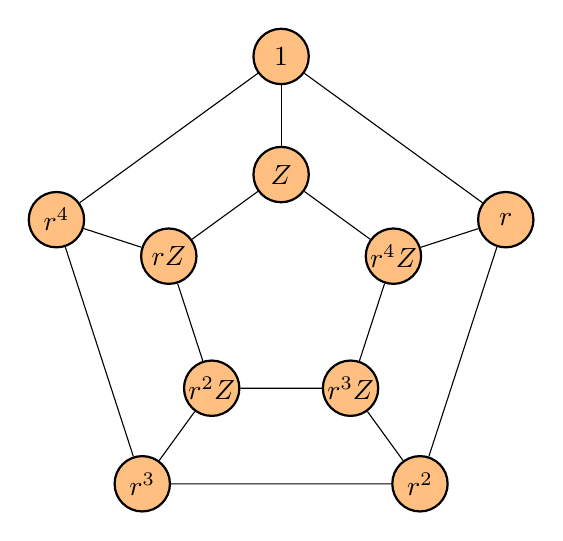
\begin{tikzpicture}[rotate=90, scale=1.5]
    \tikzset{vertex/.style={draw, thick, circle, fill=orange!50, minimum size=20pt, inner sep=0pt}}
    
    \node[vertex] (v1) at (-0*360/5:1) {$Z$};
    \node[vertex] (v2) at (-0*360/5:2) {$1$};
    \node[vertex] (v3) at (-1*360/5:1) {$r^4Z$};
    \node[vertex] (v4) at (-1*360/5:2) {$r$};
    \node[vertex] (v5) at (-2*360/5:1) {$r^3Z$};
    \node[vertex] (v6) at (-2*360/5:2) {$r^2$};
    \node[vertex] (v7) at (-3*360/5:1) {$r^2Z$};
    \node[vertex] (v8) at (-3*360/5:2) {$r^3$};
    \node[vertex] (v9) at (-4*360/5:1) {$rZ$};
    \node[vertex] (v10) at (-4*360/5:2) {$r^4$};
    
    \draw (v1) -- (v2);
    \draw (v1) -- (v3);
    \draw (v2) -- (v4);
    \draw (v3) -- (v4);
    \draw (v3) -- (v5);
    \draw (v4) -- (v6);
    \draw (v5) -- (v6);
    \draw (v5) -- (v7);
    \draw (v6) -- (v8);
    \draw (v7) -- (v8);
    \draw (v1) -- (v9);
    \draw (v7) -- (v9);
    \draw (v2) -- (v10);
    \draw (v8) -- (v10);
    \draw (v9) -- (v10);
    \end{tikzpicture}
    \end{center}
\end{primer}

\begin{definicija}\label{def_ozina}
    Številu \begin{equation*}
    \operatorname{\alpha}_{k}(G) := \min \left\{ l(w)  \middle|\,  w \in F_k \setminus \left\{ 1\right\} \text{ je zakon v } G  \right\} \cup \left\{ \infty\right\} 
    \end{equation*}  
    rečemo \emph{$k$-črkovna ožina grupe $G$}.  
    \end{definicija}
    

\begin{opomba} % TODO tole malo popravi, ni čisto logično ubesedeno
Ime ožina grupe -- ki je uporabljeno na primer v virih \cite{Schneider_2016}, \cite{Bradford_Thom_2017} in \cite{Schleimer_2001} -- je nekoliko zavajajoče. Izhaja iz Cayleyjevega grafa grupe, vsak njegov cikel $g_1 , g_2, \ldots, g_n, g_1$ namreč
podaja zvezo $s_1 s_2 \cdots s_n = 1_G$ za elemente $s_i \in S$, kjer za $i = 2, \ldots, n$ velja $s_i = g_{i - 1}^{-1} g_i$ in $s_1 = g_n^{-1} g_1$.
V kontekstu zakonov je to ime do neke mere neupravičeno, saj beseda $s_1 s_2 \cdots s_n$ ni nujno zakon v grupi. Če si pogledamo na primer grupo $C_3 \times C_5 = \langle (\xi, 1), (1, \eta) \rangle$,
bo Cayleyjev graf $\text{Cay}(C_3 \times C_5, \{ (\xi, 1)^{\pm 1} , (1, \eta)^{\pm 1} \})$ vseboval 3-cikel, ki ga porodi generator $(\xi , 1)$. Po drugi strani pa beseda $\xi^3$ očitno ni zakon v grupi $C_3 \times C_5$, ki premore element reda 5.
Ker je grupa $C_3 \times C_5$ Abelova, ni težko razmisliti, da velja $\alpha_k(C_3 \times C_5) = 4$ za $k \ge 2$ in $\alpha_1(C_3 \times C_5) = 15$. 

\end{opomba}

Izkaže se, da so najbolj zanimivi in za obravnavo relevantni dvočrkovni zakoni. To nam sporočata naslednji dve trditvi.
\begin{trditev}
\label{trd_vlozitev_proste_grupe}
 Obstaja vložitev grupe $F_{2 \cdot 3^{k}} = \langle a_1, \ldots, a_{2 \cdot 3^{k}} \rangle$ v grupo $F_2 = \langle a,b \rangle $, da velja $l(a_i) = 2k + 1$, kjer $l(w)$ označuje dolžino besede $w \in F_2 = \langle a,b \rangle$. 
\end{trditev}


\begin{dokaz}
Dokaz trditve ni posebno zahteven, vendar je nekoliko preveč tehničen za naše potrebe, saj bi zahteval uvedbo in razumevanje pojmov Schreierjevega grafa in fundamentalne grupe grafa, ki ju sicer tekom naloge ne potrebujemo. Naveden je v~\cite[str.~5]{Schneider_2016}, glavna ideja je obravnavati Cayleyev graf proste grupe $F_2$ z dvema generatorjema.
Drevo vseh besed dolžine $k$ na ustrezen način dopolnimo (do Schreierjevega grafa) tako, da dodamo povezave listom. Pri tem dobimo cikle dolžine $2k + 1$ in (s pomočjo fundamentalne grupe grafa) utemeljimo, da lahko jih lahko obravnavamo kot elemente $F_{2 \cdot 3^{k}}$, vložene v $F_2$. 
\end{dokaz}


\begin{posledica}\label{psl_veccrkovni_zakoni_meje}
Naj bo $G$ grupa in $k \ge 2$ naravno število. Potem velja \begin{equation*}
     \alpha_k(G) \le  \alpha_2(G) 
\end{equation*}  
in \begin{equation*}
\alpha_2(G) \le \left( {2 \left\lceil \log_3 \left(\frac{k}{2} \right) \right\rceil + 1  } \right) \alpha_k(G).
\end{equation*}  
\end{posledica}
\begin{dokaz}
    Prva neenakost je očitna, saj so vsi dvočrkovni zakoni tudi $k$-črkovni zakoni. Druga neenakost drži, saj lahko po prejšnji trditvi vložimo $F_{{2 \left\lceil \log_3(\frac{k}{2}) \right\rceil}}$ v $F_2$
    tako, da noben generator ni daljši od ${2 \left\lceil \log_3(\frac{k}{2}) \right\rceil + 1  }$. Hkrati velja $F_k \subseteq F_{{2 \left\lceil \log_3(\frac{k}{2}) \right\rceil}}$, kar nam da želeno neenakost.
\end{dokaz}


\subsection{Teorija naključnih sprehodov}

Za obravnavo zakonov v simetričnih grupah bomo potrebovali naključne sprehode, natančneje lene naključne sprehode (TODO poglej, če se res tako imenuje).
Naj bo $G$ grupa, generirana s simetrično podmnožico $S \subseteq G$. Tekom tega razdelka naj bo $\Gamma = \operatorname{Cay}(G, S)$, ki je po prejšnjem premisleku 



\begin{definicija}
\label{def_leni_nakljucni_sprehod}
    Leni naključni sprehod je naključno zaporedje elementov $w_n \in S$ za $n \in \mathbb{N} \cup \left\{ 0\right\} $, porojeno s formulo \begin{equation*}
        \mathbb{P}(w_{n+1} = g   \vert \,  w_n = h) = \begin{cases}
            \frac{1}{2}; & \text{če }  g = h, \\
            \frac{1}{2 \lvert S \rvert }; & \text{če } g = sh \text{ za neki } s \in S.
        \end{cases}
    \end{equation*}  
\end{definicija}
Na vsakem koraku lenega naključnega sprehoda se torej z verjetnostjo $1 / 2$ element ne spremeni, z verjetnostjo $1 / 2$ pa se naključno spremeni v enega od svojih sosedov, ki jih je $\lvert S \rvert$.
To lahko opišemo tudi z matrikami. Recimo, da je $u_n$ vejretnostna porazdelitev $\lvert G \rvert$ razsežnega vektorja, ki predstavlja vozlišča grafa $\Gamma$, po $n$-tem koraku in recimo, da začetno porazdelitev $u_0$ poznamo. Dalje, definiramo matriko lenega naključnega sprehoda $M \in M_{\lvert G \rvert }(\mathbb{R})$, s predpisom    
\begin{equation*}
M = \frac{1}{2} \left(I + \frac{1}{\lvert S \rvert } A \right) = \frac{1}{2} (I + \tilde{A}),
\end{equation*}  
kjer smo z $A$ označili matriko soseščine grafa $\Gamma$, z $\tilde{A}$ pa smo označili matriko $\frac{1}{\lvert S \rvert} A$, da . Ni težko premisliti, da po definiciji \ref{def_leni_nakljucni_sprehod} sledi zveza 
\begin{equation*}
u_n = M^{n} u_0,
\end{equation*}  
ki nam omogoča vpogled v lastnosti naključnih sprehodov. 

\begin{lema}
\label{lem_M_je_sebiadjungirana}
Matrika $M$ je diagonalizabilna, sebiadjungirana in njene lastne vrednosti ležijo v intervalu $[0, 1]$.
\end{lema}
\begin{dokaz}
Ker je realna matrika $M$ simetrična, je diagonalizabilna, sebiadjungirana in velja, da so vektorji, ki pripadajo paroma različnim lastnim vrednostim, med seboj ortogonalni. Enako velja za matriko $A$. Sebiadjungiranost nam implicira realnost lastnih vrednosti matrik $M$ in $A$.
Z oceno matričnih norm \begin{equation*}
    \sqrt{ \lambda_{\max} (\tilde{A}^2)} = \sqrt{\lambda_{\max} (\tilde{A}^{T} \tilde{A} )}  = \lvert\lvert \tilde{A} \rvert\rvert_2 \le \sqrt{\lvert\lvert A \rvert\rvert_1}  \lvert\lvert \tilde{A} \rvert\rvert_{\infty} = 1 
\end{equation*}  
sledi, da ima matrika $\tilde{A}$ lastne vrednosti v intervalu $[-1 ,1]$, kar pomeni, da lastne vrednosti matrike $M$ ležijo v intevalu $[0, 1]$. 
\end{dokaz}

Ker vemo, da so vse lastne vrednosti realne, jih lahko po razvrstimo po velikosti: 
\begin{equation*}
1 \ge \lambda_1(G, S) \ge \lambda_2(G, S) \ge \ldots \ge \lambda_{\lvert G \rvert }(G, S).  
\end{equation*}  
Izkaže se, da je glede na izbiro grupe $G$ in njene generirajoče množice $S$ lastna vrednost $\lambda_1(G, S) = 1 > \lambda_2(G, S)$. (TODO, posledica tega, da je $\Gamma$ povezan + konvergence zaporedja)
Razliko $1 - \lambda_2(G, 2)$ imenujemo \emph{spektralna razlika} grafa $\Gamma$. 

\begin{definicija}
\label{def_diameter_cayleyjevega_grafa}
Diameter Cayleyjevega grafa $\Gamma = \operatorname{Cay}(G, S)$ je število \begin{equation*}
    \operatorname{diam}(G, S) := \min \left\{ n \in \mathbb{N}  \middle|\, \forall g \in G. \exists s_1, \ldots , s_n \in S \cup \left\{ 1_G \right\} . g = s_1 \cdots s_n \right\} 
\end{equation*}  
\end{definicija}
Intuitivno nam diameter Cayleyjevega grafa poda najmanjše število korakov, po katerem lahko naključni sprehod po grafu $\Gamma$ doseže poljubni element grupe $G$. Za vse končnogenerirane in posledično končne grupe je diameter dobro definiran.
Za ocenjevanje dolžin zakonov v grafih je bistvena sledeča zveza med diametrom grafa in spektralno razliko lenega naključnega sprehoda.

\begin{trditev}
\label{trd_zveza_med_diametrom_grafa_in_spektralno_razliko}
 Velja zveza \begin{equation*}
 1 - \lambda_1(G, S) \ge \frac{1}{2 \lvert S \rvert \operatorname{diam}(G, S)^2}.
 \end{equation*}  
\end{trditev}
\begin{dokaz}
% TODO najdi referenco za dokaz te leme, oz si poglej vir, na katerega se sliče Thom
\end{dokaz}

Od tod sledi pomembna posledica \begin{posledica}
\label{psl_posledica_zveze_diameter}
Naj bo vektor $u = \frac{1}{\lvert G \rvert} I$ in naj bo $e_1$ bazni vektor enote $1_G$ (TODO tole bolje razloži). Potem velja ocena \begin{equation*}
\lvert M^{n} e_1 - u \rvert \le \lambda_1(G, S)^{n} \le \left( 1 - \frac{1}{2 \lvert S \rvert \operatorname{diam}(G, S)^2 } \right)^{n}. 
\end{equation*}    
\end{posledica}
\begin{dokaz}
Desna neenakost je direktna posledica trditve \ref{trd_zveza_med_diametrom_grafa_in_spektralno_razliko}. (TODO zakaj leva stran enačbe ... to bi se moralo dati intuitivno dokazati )
\end{dokaz}

Za konec potrebujemo še zadnjo lemo. 
\begin{lema}\label{lem_posledica_neenakosti_csb}
Naj bo $E$ podmnožica grupe $G$ in naj bo $\alpha := \lvert E \rvert / \lvert G \rvert$ in naj bo $(w_n)_{n \in  \mathbb{N}}$ leni naključni sprehod.
Če velja ocena \begin{equation*}
n \ge 2 \lvert S \rvert \operatorname{diam}(G, S)^2 \log(2 \lvert G \rvert ), 
\end{equation*}  
    velja $\mathbb{P}(w_n \in E) \ge \alpha / 2$.
\end{lema}  
\begin{dokaz}
TODO, to je Cauchy--Schwarz
\end{dokaz}

% TODO tukaj poveži besedilo z intuitivno razloago

Glavni rezultat, ki bo zagotovil obstoj kratkih zakonov v simetričnih grupah, je Helfgott--Seressov izrek, ki omeji diameter Cayleyjevih grafov simetričnih grup, generiranih s parom elementov. \begin{izrek}[Helfgott--Seress]\label{izr_Helfgott_Seress}
Naj par $(\sigma, \tau) \in S_n^2$ generira grupo $S_n$, torej $\langle \sigma, \tau \rangle = S_n$. Potem obstaja konstanta $C > 0$, da je diameter grafa $\Gamma = \operatorname{Cay}(S_n, \left\{ \sigma^{\pm 1}, \tau^{\pm 1} \right\} )$ največ 
\begin{equation*}
\exp(C \log(n)^{4} \log(\log(n))).
\end{equation*}
\end{izrek}  
Dokaz tega izreka je zelo težek in se močno nanaša na klasifikacijo končnih enostavnih grup, zato ga opuščamo. Bralec ga lahko najde v članku \cite{Helfgott_Seress_2013}.



\section{Komutatorska in razširitvena lema}

\subsection{Komutatorska lema}



Recimo, da poznamo zakone v nekaterih podmnožicah grupe $G$, zanima pa nas, kako bi iz njih zgradili zakone V večjih podmnožicah te grupe. Na to vprašanje odgovarjata komutatorska in razširitvena lema,
ki sta ključni orodji pri obravnavi zakonov. Začeli bomo z dokazom komutatorske leme, za katerega bomo potebovali nekaj definicij.

\begin{definicija}
    \label{def_izginjajoca_mnozica}
    Naj bo $G$ grupa in $w \in  F_k$. Potem množico \begin{equation*}
    Z(G, w) := \left\{ (g_1, .., g_{k}) \in  G^{k}  \middle|\, w(g_1, \ldots, g_{k}) = 1_G \right\} 
    \end{equation*}  
    imenujemo \emph{izginajoča množica besede $w$ v grupi $G$}. Tu $w(g_1, \ldots, g_{k})$ označuje evalvacijo besede $w$ z elementi $g_1, \ldots, g_n$, v skladu z notacijo na začetku razdelka \ref{sec_osnovne_lastnosti_zakonov}.  
    \end{definicija}



% \begin{definicija}\label{def_aperiodicna_beseda}
%     Naj bo $G$ grupa. Element $g \in  G$ je netrivialna potenca, če obstajata $h \in G$ in naravno število $n > 1$, da je $g = h^{n}$.
% \end{definicija}

% \begin{lema}[\cite{Lyndon_Schupp_2015}[str.~8, trditev 2.6]]\label{lem_uporaba_nielsen}
% Vsaka končnogenerirana podgrupa proste grupe je prosta.   
% \end{lema}
% % \begin{skica}
% %     -najprej Nielsenove transformacije
% %     -nato N-okrajšanost
% %     -ideja, da lahko prevedeš vse U na N-okrajšane
% %     -lema, da N-okrajšane ravno pravšnje
% % Ta lema je posebni primer Nielsen-Schreierjevega izreka, ki trdi, da je vsaka podgrupa proste grupe prosta \cite{Lyndon_Schupp_2015}[str.~8, trditev 2.11]. Njen dokaz je podan na straneh 5--7 v istega vira,  

% % \end{skica}

% Ta lema je posebni primer klasičnega Nielsen--Schreierjevega izreka, ki pravi, da je vsaka podgrupa proste grupe prosta. Dokazana je v \cite{Lyndon_Schupp_2015}[5--7] z uporabo Nielsenovih transformacij. 

\begin{lema}
\label{lem_posledica_nielsen_schreier}
Naj bosta $w_1, w_2 \in F_2 = \langle a, b \rangle$ besedi. Potem velja natanko ena izmed naslednjih trditev. \begin{enumerate}
    \item Besedi $w_1$ in $w_2$ komutirata in imata isto osnovo: Obstaja element $c \in F_2$ ter števili $k_1, k_2 \in \mathbb{Z}$, da velja $w_1= c^{k_1}$ in $w_2 = c^{k_2}$. 
    \item Podgrupa $\langle w_1, w_2 \rangle \subseteq F_2 = \langle a, b \rangle$ je izomorfna prosti grupi $F_2$.
\end{enumerate}
\end{lema}
\begin{dokaz}
    Po Nielsen--Schreierjevem izreku \ref{izr_nielsen_schreier} vemo, da je $F:= \langle w_1 , w_2 \rangle \le F_2$ prosta grupa. Preslikava $\varphi : F_2 = \langle a, b \rangle \to F$,
    inducirana s preslikavama $a \mapsto w_1$, $b \mapsto w_2$, je očitno epimorfizem. Od tod po trditvi \ref{trd_enolicnost_prostih_grup} sledi, da je $F$ generirana z enim ali dvema elementoma.
    V prvem primeru je $F = \langle c \rangle$ za neko besedo $c \in F_2$, od koder sledi $w_1= c^{k_1}$ in $w_2 = c^{k_2}$ za neki celi števili $k_1$ in $k_2$. V tem primeru besedi $w_1$ in $w_2$ očitno komutirata.
    V drugem primeru je $F$ po trditvi \ref{trd_enolicnost_prostih_grup} izomorfna prosti grupi $F_2$.
\end{dokaz}
Preden se lotimo komutatoske leme, uvedimo še naslednjo definicijo.
\begin{definicija}\label{def_aperiodicna_beseda}
    Naj bo $G$ grupa. Element $g \in  G$ je \emph{periodičen}, če je oblike $g = h^{n}$ za neki element $h \in G$ in število $n \in \mathbb{Z} \setminus \{ 0, \pm 1 \}$. Sicer rečemo, da je $g$ \emph{aperiodičen}.
    \end{definicija}
Osnovna ideja komutatorske leme je pravzaprav preprosta. Recimo, da imamo besedi $w_1, w_2 \in F_2 \setminus \left\{ 1_{F_2}\right\}  = \langle a,b \rangle$, ki jima pripadata izginjajoči množici $Z(G, w_1)$ ter $Z(G, w_2)$.
oglejmo si komutator $w = [w_1, w_2]$. Če vzamemo par $(g, h) \in Z(G, w_1)$, bo veljalo \begin{equation*}
w(g,h) = [w_1(g,h), w_2(g,h)] = [1_{F_2}, w_2(g,h)] = 1_{F_2}.
\end{equation*}  
  Seveda velja simetrično tudi za pare druge izginjajoče množice. Od tod sledi sklep \begin{equation*}
  Z(G, [w_1, w_2]) \supseteq Z(G, w_1) \cup Z(G, w_2).
  \end{equation*}  
Glavni problem, na katerega lahko naletimo pri takšnem združevanju besed, je potencialna trivialnost komutatorja $[w_1, w_2]$, ki bi ustrezala trivialnemu zakonu.
Po lemi \ref{lem_posledica_nielsen_schreier} je komutator $[w_1, w_2]$ trivialen natanko tedaj, ko sta besedi $w_1$ in $w_2$ periodični z isto osnovo. 
Komutatorska lema podaja konstrukcijo, ki preprečuje pojav takšnih zapletov. V sledeči obliki se pojavi v članku \cite{Kozma_Thom_2016} in magistrskem delu \cite{Schneider_2016}, po katerem so prirejeni dokazi.

\begin{lema}
    \label{lem_komutatorska_lema}
     Naj bo $k \ge 2$, $e \in  \mathbb{N}$ in naj bodo besede $w_1, \ldots, w_m \in F_k$ netrivialne, pri čemer je $m = 2^{e}$. Potem obstaja aperiodična beseda $w \in F_k$
     dolžine \begin{equation*}
     l(w) \le 2m \left(m + \sum_{i=1}^{m} l(w_{i}) \right),
     \end{equation*}  
    da za vsako grupo $G$ velja \begin{equation*}
    Z(G, w) \supseteq \operatorname{Z}(G, w_1) \cup \ldots \cup \operatorname{Z}(G, w_m).
    \end{equation*}       
\end{lema}
    \begin{dokaz}
        Dokaz poteka z indukcijo po $e \in  \mathbb{N}$. Naj bo $F_k = \langle a_1, \ldots , a_{k} \rangle = \langle S \rangle$.  Za $e = 0$ (oziroma $m = 1$) vzamemo $w = [s, w_1]$, kjer je $s \in S$ takšna črka, da beseda $w_1$ ni periodična z osnovo $s$. 
        To lahko zaradi pogoja $k \ge 2$ vedno storimo. Zaradi ustrezne izbire je komutator $[s, w_1]$ po lemi \ref{lem_posledica_nielsen_schreier} aperiodičen z dolžino največ $2(l(w_1)  + 1)$.
        Kot smo videli v predhodnem razmisleku, za poljubno grupo $G$ velja $\operatorname{Z}(G, w) \supseteq \operatorname{Z}(G, s) \cup \operatorname{Z}(G, w_1)$.
        
        Zdaj se lotimo indukcijskega koraka v primeru $e \ge 1$ oziroma $m \ge 2$. Naj bodo podane besede $w_1, \ldots, w_{m / 2}, w_{m / 2 + 1}, \ldots, w_{2m}$. Po indukcijski predpostavki obstajata aperiodični besedi $v_1, v_2 \in  F_{k}$,  da velja
        \begin{equation*}
        l(v_1) \le m \left(\frac{m}{2} + \sum_{i=1}^{m / 2} l(w_{i}) \right), \,\,\, l(v_2) \le m \left(\frac{m}{2} + \sum_{i= m / 2 + 1}^{m} l(w_{i}) \right)
        \end{equation*}  
        in \begin{equation*}
        \operatorname{Z}(G, v_1) \supseteq \operatorname{Z}(G, w_1) \cup \ldots \cup \operatorname{Z}(G, w_{m / 2}),
        \end{equation*}  
        \begin{equation*}
            \operatorname{Z}(G, v_2) \supseteq \operatorname{Z}(G, w_{m / 2 + 1}) \cup \ldots \cup \operatorname{Z}(G, w_{m})
        \end{equation*}  
        za vsako grupo $G$.

        Zdaj moramo le še ugotoviti, kako lahko besedi $v_1$ ter $v_2$ ustrezno združimo. Po lemi \ref{lem_posledica_nielsen_schreier} vemo, da bo komutator $[v_1, v_2]$ trivialen natanko v primeru $v_1 = v_2^{\pm 1}$, ker sta $v_1$ in $v_2$ po predpostavki aperiodični. V primeru, da sta periodični, imamo \begin{equation*}
        \operatorname{Z}(G, w_1) = \operatorname{Z}(G, w_2)
        \end{equation*}  
         in lahko nastavimo $w := v_1$ ali $w := v_2$, pri čemer je pogoj na dolžino besede $w$ očitno izpolnjen. Če imamo $v_1 \neq v_2^{\pm 1}$, nastavimo $w := [v_1, v_2]$. V tem primeru je beseda $w$ aperiodična, kot je razloženo v viru \cite{Schutzenberger_1959}. Tega rezultata ne bomo podrobneje predstavili, saj bi lahko aperiodičnost
         zagotovili na enak način kot v indukcijskem koraku z minimalno slabšim rezultatom. Indukcijska predpostavka nam zagotavlja 
         \begin{equation*}
         l(w) \le 2m  \left(\frac{m}{2} + \sum_{i=1}^{m / 2} l(w_{i}) \right) + 2m \left(\frac{m}{2} + \sum_{i= m / 2 + 1}^{m} l(w_{i}) \right) = 2m \left( m + \sum_{i = 1}^{m} l(w_{i}) \right).
         \end{equation*}
    \end{dokaz}

Lemo brez težav posplošimo tudi na število besed, ki ni dvojiška potenca.
\begin{lema}
\label{lem_komutatorska_lema_splosna}
Naj bo $k \ge 2$ in naj bodo podane netrivialne besede $w_1, \ldots, w_{m} \in  F_m$. Potem obstaja aperiodična beseda $w \in F_k$ dolžine \begin{equation*}
l(w) \le 8m \left(m +  \sum_{i = 1}^{m} l(w_{i}) \right),
\end{equation*}  
da za vsako grupo $G$ velja \begin{equation*}
\operatorname{Z}(G, w) \supseteq \operatorname{Z}(G, w_1) \cup \ldots \cup  \operatorname{Z}(G, w_{m}).
\end{equation*}    
\end{lema}

% To lemo sem v praktično enaki obliki uspel dokazati na bolj elementaten način v obliki leme \ref{lem_komutatorska_lema_splosna}, brez uporabe Nielsenovega izreka.
% Ideja za dokaz leme \ref{lem_komutaroska_lema_nova} izvira iz dokaza leme 2 v \cite[str.~7--8]{Schneider_2016}.  

% \begin{lema}
% \label{lem_komutaroska_lema_nova}
% Naj bo $G$ grupa, $H_i \subseteq  G$ njene simetrične podmnožice ($H_i = H_i ^{-1}$), in naj bo za vsak $i  \in \{1, \ldots, 2^{e}\}$ beseda $w_{i} \in F_k$ zakon v podmnožici $H_i$. Potem obstaja beseda $w \in F_k$ dolžine \begin{equation*}
% l(w) \le  m \sum_{i = 1}^{n} l(w_i),
% \end{equation*}  
% za katero velja $H_1 \cup  \ldots \cup H_m \subseteq  Z(G, w)$, torej je zakon v vseh podgrupah $H_i$. 
% \end{lema}
% \begin{dokaz}
% Dokaz poteka z indukcijo po $e \in  \mathbb{N}$ za primer $k = 2$, za $k \ge 3$ je dokaz praktično enak oziroma lažji. Naj bo $F_2 = \langle a , b \rangle$. Za $e = 0$ (oziroma $m = 1$) vzamemo zadostuje $w$, njena dolžina je $l(w_1)$, za poljubno grupo $G$ velja $\operatorname{Z}(G, w) \supseteq \operatorname{Z}(G, w_1)$. 
%         Zdaj se lotimo indukcijskega koraka v primeru $e \ge 1$ oziroma $m \ge 2$. Naj bodo podane besede $w_1, \ldots, w_{m / 2}, w_{m / 2 + 1}, \ldots, w_{m}$. Po indukcijski predpostavki obstajata besedi $v_1, v_2 \in  F_{2}$, da velja
%         \begin{equation*}
%         l(v_1) \le \frac{m}{2} \sum_{i=1}^{m / 2} l(w_{i}) , \,\,\, l(v_2) \le \frac{m}{2} \sum_{i= m / 2 + 1}^{m} l(w_{i})
%         \end{equation*}
%         in \begin{equation*}
%         \operatorname{Z}(G, v_1) \supseteq \bigcup_{i = 1}^{m / 2} H_i^2, \,\,\,  \operatorname{Z}(G, v_2) \supseteq \bigcup_{i = m / 2 + 1}^{m} H_i^2,
%         \end{equation*}  
%         za vsako grupo $G$. 
%         Zdaj moramo le še utemeljiti, da lahko besedi $v_1$ ter $v_2$ ustrezno združimo. Če bi takoj definirali $w = [v_1, v_2]$, bi v primeru $v_1 = v_2^{\pm 1}$ namreč dobili trivialno besedo, česar si ne želimo.
%         Zato obravnavajmo besedi $v_1$ in $v_2$ glede na to, s katero črko se začneta oziroma končata. Za lažjo notacijo bomo pisali, da je beseda element $V_{s_1 s_2}$, če se začne s črko $s_1 \in \left\{ a^{\pm 1}, b^{\pm 1} \right\}$ in konča s črko $s_2 \in \left\{ a^{\pm 1}, b^{\pm 1}\right\}$.   
%         Uvedimo še bijekciji $\tau, \kappa: F_2 \to F_2$, porojeni s predpisi $\tau: a \mapsto a^{-1} , b \mapsto b$ in $\kappa: a \mapsto b, b \mapsto a$. Ni težko preveriti, da z njima lahko vse besede prevedemo na eno izmed oblik $V_{ab}$, $V_{aa}$ ali $V_{aa^{-1}}$. Na primer za besedo $ba^{-1} \in V_{ba^{-1}}$ velja $\tau(\kappa(ba^{-1})) = ab \in V_{ab}$ in podobno za ostale.
%         Najprej besedi $v_1$ in $v_2$ prevedemo na besedi $v_1'$ in $v_2'$, ki sta ene izmed treh oblik. Nato ju z ustrezno uporabo preslikav $\tau$ in $\kappa$ pretvorimo v besedi $v_1''$ in $v_2''$ tako, da komutator $w = [v_1'', v_2'']$ gotovo ne bo trivialen.
%         \begin{enumerate}
%             \item V primeru $v_1', v_2' \in V_{aa } \cup V_{a a^{-1}}$ nastavimo $v_{2}'' = \kappa(v_2)$.
%             \item V primeru $v_1' \in V_{aa}, v_2' \in V_{ab}$ ne pride do krajšanja, imamo namreč \begin{equation*}
%                 [v_1', v_2'] =  [a \ldots a, a \ldots b] = a \ldots a a \ldots b a^{-1} \ldots a^{-1} b ^{-1} \ldots a.
%             \end{equation*}  
%             \item V primeru $v_1' \in V_{ab}, v_2' \in V_{aa}$ ne pride do krajšanja, imamo namreč  \begin{equation*}
%                 [v_1', v_2'] = [a \ldots b, a \ldots a] = a \ldots b a \ldots a b^{-1} \ldots a^{-1} a ^{-1} \ldots a^{-1}.
%             \end{equation*}
%             \item V primeru $v_1' \in V_{aa^{-1}}, v_2' \in V_{ab}$ nastavimo $v_2'' = \kappa(v_2)$, imamo namreč \begin{equation*}
%                 [v_1', v_2''] =  [a \ldots a^{-1}, b \ldots a] = a \ldots a^{-1} b \ldots a a \ldots a^{-1} a ^{-1} \ldots b^{-1}.
%             \end{equation*}
%             \item V primeru $v_1' \in V_{ab}, v_2'' \in V_{aa^{-1}}$ nastavimo $v_2'' = \tau(v_2)$, imamo namreč \begin{equation*}
%                 [v_1', v_2''] =  [a \ldots b, a^{-1} \ldots a] = a \ldots b a^{-1} \ldots a b^{-1} \ldots a^{-1} a ^{-1} \ldots a.
%             \end{equation*}
%             \item V primeru $v_1', v_2'' \in V_{ab}$ nastavimo $v_2'' = \kappa(v_2)$, imamo namreč \begin{equation*}
%                 [v_1', v_2''] =  [a \ldots b, b \ldots a] = a \ldots b b \ldots a b^{-1} \ldots a^{-1} a ^{-1} \ldots b^{-1}.
%             \end{equation*}  
%         \end{enumerate}
%         Po zgornjem razmisleku dobimo besedo oblike $w = [v_1'', v_2'']$, treba je le še razmisliti, da velja $Z(G, w) \supseteq \bigcup_{i = 1}^{m} H_i^2$. Po indukcijski prepodstavki vemo, da je \begin{equation*}
%         Z(G, v_1) \supseteq \bigcup_{i = 1}^{m / 2} H_i^2, \,\,\,  Z(G, v_2) \supseteq \bigcup_{i = m / 2 + 1}^{m} H_i^2,
%         \end{equation*}  
%         velja pa tudi \begin{equation*}
%             Z(G, v_1'') \supseteq \bigcup_{i = 1}^{m / 2} H_i^2, \,\,\,  Z(G, v_2'') \supseteq \bigcup_{i = m / 2 + 1}^{m} H_i^2,
%         \end{equation*}  
%           saj za poljubno besedo $u \in F_2$, ki je zakon v simetrični podmnožici $H_u \subseteq G$, velja (zaradi simetričnosti $H_u$) $Z(G, u) \cap  Z(G, \tau(u)) \supseteq H_u ^2$, hkrati pa vedno velja $Z(G, u) = Z(G, \kappa(u))$.
%         Z besedami, preslikavi $\tau$ in $\kappa$ ohranjata lastnost, da je beseda zakon v simetrični podmnožici grupe. 
%           Indukcijska predpostavka nam zagotavlja 
%          \begin{equation*}
%          l(w) \le m  \sum_{i=1}^{m / 2} l(w_{i}) + m \sum_{i= m / 2 + 1}^{m} l(w_{i})  = m \sum_{i = 1}^{m} l(w_{i}) .
%          \end{equation*}
% \end{dokaz}

% \begin{lema}
% \label{lem_komutatorska_lema_splosna}
% Naj bo $G$ grupa in naj bodo $w_{i} \in F_k$ netrivialne besede za $i \in \left\{ 1, \ldots, m \right\}$. Potem obstaja aperiodična beseda $w \in F_k$ dolžine \begin{equation*}
%     l(w) \le  8 m (m + \sum_{i = 1}^{m} l(w_i)),
%     \end{equation*}  
%     za katero velja $Z(G, w_1) \cup  \ldots \cup Z(G, w_m) \subseteq  Z(G, w)$.
% \end{lema}


\begin{dokaz}
    Naj bo $e$ takšno naravno število, da velja $m \le 2^{e} < 2m$. Nastavimo \begin{equation*}
    w_1' := w_1, \ldots, w_{m}' := w_{m}, w_{m+1}' := w_1, \ldots, w_{2^{e}}' := w_{2^{e} - m}. 
    \end{equation*}
    Ker velja $m < 2m$ in $\sum_{i = 1}^{2^{e}} w_i' \le 2 \sum_{i = 1}^{m} l(w_i)$, želena ocena sledi z uporabo leme \ref{lem_komutatorska_lema}.  
\end{dokaz}


Ta rezultat lahko nekoliko omilimo, da dobimo bolj praktično oceno.
\begin{posledica}
\label{psl_komutatorska_lema_prakticna}
Naj bo $k \ge 2$ in naj bodo podane netrivialne besede $w_1, \ldots, w_m \in  F_k$. Potem obstaja aperiodična beseda $w \in  F_k$ dolžine \begin{equation*}
l(w) \le 8m^2 \left(1 +  \max_{i = 1, \ldots, m} l(w_i) \right)
\end{equation*}      
\end{posledica}
\begin{dokaz}
    To je direktna posledica leme \ref{lem_komutatorska_lema_splosna} skupaj z dejstvom, da je \begin{equation*}
    \sum_{i = 1}^{m} l(w_{i}) \le m \max_{i = 1, \ldots, m} l(w_i).
    \end{equation*}  
\end{dokaz}


\begin{primer}\label{prm_komutatorska_produkt_elementov}
Najelegantnejša uporaba komutatorske leme se pojavi pri obravnavi grupe kot direktnega produkta. Naj bo recimo $G := C_5 \times D_{10}$. 
V podgrupi $C_5$ imamo zakon $a^{5} \in F_2 = \langle a, b \rangle $ dolžine $5$, razširitvena lema \ref{lem_razsiritvena_lema} pa nam bo povedala, da obstaja zakon $a^2 b^2 a^{-2} b^{-2}$ v $D_{10}$, ki je dolžine 8. Po lemi \ref{lem_komutatorska_lema} torej obstaja
netrivialna beseda $w \in F_2$ dolžine največ $2 \cdot 2 (2 + 5 + 8) = 60$, ki je zakon v grupi $G$.
\end{primer}
\begin{primer}\label{prm_komutatorska_redi_elementov}
Naj bo $G$ grupa. Recimo, da red vsakega njenega elementa deli vsaj eno izmed naravnih števil $n_1 \ldots, n_m$. Če za vsak $i = 1, \ldots , m$ uvedemo množico $H_{n_i} := \{ g \in G \vert g^{n_i} = 1_G \}$,
očitno velja, da je $\bigcup_{i = 1}^m H_{n_i} = G$. Ker za vsak $i$ velja $Z(G, a^{n_i}) = H_{n_i} \times G$, lahko s pomočjo komutatorske leme \ref{psl_komutatorska_lema_prakticna} združimo besede $a^{n_i}$ v besedo $w$ dolžine
\begin{equation*}
    l(w) \le 8 m^2 \left( 1 + \max_{i = 1, \ldots, m} n_i \right),
\end{equation*}
ki je zakon v grupi $G$, saj velja \begin{equation*}
    Z(G, w) \supseteq \bigcup_{i = 1}^m Z(G, a^{n_i}) =  \bigcup_{i = 1}^m H_{n_i} \times G = G \times G.
\end{equation*}\end{primer}
Čeprav sta ta primera razmeroma enostavna, sta ključna pri praktično vseh konstrukcijah zakonov, kar bomo videli recimo na koncu razdelka \ref{sec_grupe_psl2q} pri obravnavi družine grup $\operatorname{PSL}_2(q)$. 


% Definirajmo namreč grupo \begin{equation*}
% \Gamma_n = \prod_{G \text{ grupa},\, \lvert G \rvert \le n }  G 
% \end{equation*}  
  


\subsection{Razširitvena lema}

Nekoliko bolj povezana s strukturo grup je razširitvena lema. Za njeno formulacijo najprej definirajmo kratka eksaktna zaporedja.
\begin{definicija}
\label{def_kratko_eksaktno_zaporedje}
Naj bodo $A, B, C$ grupe in naj $\mathbf{1}$ označuje trivialno grupo. Kratko eksaktno zaporedje je zaporedje homomorfizmov
\begin{equation*}
\mathbf{1} \to A \xrightarrow{\varphi} B \xrightarrow{\psi} C \to \mathbf{1},
\end{equation*}  
kjer je $\ker \psi = \operatorname{im} \varphi$, $\varphi$ je injektivni in $\psi$ surjektivni homomorfizem.
\end{definicija}


\begin{lema}\label{lem_razsiritvena_lema}
    Naj bo $N$ edinka v grupi $G$ in naj bosta $i : N \to G$ inkluzija ter $\pi : G \to G / N$ kanonična projekcija. To lahko zapišemo z naslednjim kratkim eksaktnim zaporedjem. \begin{equation*}
        \mathbf{1} \to N \xrightarrow{i} G \xrightarrow{\pi} G / N \to  \mathbf{1}  
    \end{equation*}  
    Naj bo $F_k = \langle a_1, \ldots, a_k \rangle  = \langle S \rangle$. Naj bo $w_N \in F_k$ netrivialni zakon v grupi $N$ in $w_{ G / N} \in  F_k$ netrivialni zakon v kvocientu $G / N$. 
    Potem obstaja netrivialni $k$-črkovni zakon v grupi $G$ dolžine kvečjem $l(w_N) l( w_{ G / N } )$.
\end{lema}
\begin{dokaz}
    Dokaz je prirejen po \cite[str.~10]{Schneider_2016} in obravnava dva možna primera oblike zakona $w_{ G / N }$. 
     V prvem primeru je $w_{ G / N }$ enočrkovni zakon, torej je oblike $w_{G / N} = s^{n}$ za neko črko $s \in S$ in neničelno celo število $n$. V tem primeru je za vsak $i = 1, \ldots, k$ beseda $a_i^n$ zakon v kvocientu $G / N$. Definirajmo besedo \begin{equation*}
        w := w_N(a_1^{n}, \ldots, a_{k}^{n}).
        \end{equation*}  
        Ker je za vsak $i = 1, \ldots, k$ beseda $a_i^n$ zakon v kvocientu, preslikava $g \mapsto g^n$ vse elemente iz $G$ slika v elemente edinke $N$. Ker je $w_N$ netrivialni zakon v grupi $N$ in med paroma različnimi besedami $a_i^n$ ne more priti do krajšanja,
        je beseda $w$ netrivialni zakon v grupi $G$.
        
        Če $w_{G / N}$ ni enočrkovni zakon, lahko brez škode za splošnost predpostavimo, da je oblike $w_{ G / N} = a_1 w_{ G / N}' a_2$, kjer se $w_{ G / N}'$ niti ne začne z $a_1^{-1}$ niti ne konča z $a_2^{-1}$.
        To storimo z zaporednim izvajanjem enega izmed treh korakov: \begin{itemize}
            \item Če je zakon $w_{ G / N}$ oblike $a_1 w_{ G / N}' a_1$, ga konjugiramo s črko $a_1$ tolikokrat, da se zadnja črka razlikuje od $a_1$.
            \item Če je zakon oblike $w_{ G / N}$ oblike $a_1 w_{ G / N}' a_1^-1$, ga konjugiramo s črko $a_1^{-1}$, s čimer zmanjšamo problem.
            \item Če zakon ni ene izmed zgornjih dveh oblik, izvedemo takšno bijektivno transformacijo črk, da se beseda začne z $a_1$ in, če je le mogoče, konča z $a_2$. To transformacijo nam inducira univerzalna lastnost prostih grup. 
        \end{itemize}
        Pri tem se zavedajmo, da zakoni v grupi tvorijo karakteristično edinko proste grupe $F_k$ (razmislek pod definicijo \ref{def_zakon_formalna}), zato je uporaba zgoraj naštetih transformacij legitimna. 
        Nato definiramo besede \begin{equation*}
   w_i := w_{ G / N}(a_{i}, \ldots, a_{k}, a_1, \ldots, a_{i - 1}).
   \end{equation*}  
   Ni težko preveriti, da so netrivialni produkti besed $w_i$ -- torej $w_{i} w_{j}$, $w_{i}^{-1} w_{j}$, \\ 
   $w_{i}^{-1} w_{j}^{-1}$,  $w_{i} w_{j}^{-1}$, $w_{i} w_{i}$, $w_{i}^{-1} w_{i}^{-1}$ za vse paroma različne $i,j \in \left\{ 1, \ldots, k \right\}$ -- okrajšane.
   Zato je \begin{equation*}
    w := w_N (w_1, \ldots, w_{k})
    \end{equation*}  
    netrivialni zakon v grupi $G$. Vse besede $w_{i}$ namreč inducirajo preslikave, ki $G$ slikajo v $N$, $w_N$ pa je netrivialni zakon v $N$.       
\end{dokaz}

\begin{primer}\label{prm_razsiritvena}
    S pomočjo razširitvene leme lakho dokažemo, da za vsak $n \in \mathbb{N}$ obstaja zakon $w \in F_2$ dolžine $8$ v diedrski grupi $D_{2n}$. Ker ima podgrupa $\langle r \rangle \subseteq D_{2n}$ indeks 2, je edinka,
    zato lahko tvorimo kratko eksaktno zaporedje \begin{equation*}
        \mathbf{1} \to \langle r \rangle  \xrightarrow{i} D_{2n} \xrightarrow{\pi} D_{2n} / \langle r \rangle  \to \mathbf{1}.
        \end{equation*}
        Ker je podgrupa $\langle r \rangle$ Abelova, je v njej zakon beseda $[a, b] = aba^{-1} b^{-1}$, grupa $D_{2n} / \langle r \rangle$ pa je moči $2$ in je zato v njej zakon beseda $a^2$. Po lemi \ref{lem_razsiritvena_lema} torej obstaja beseda $w \in F_2$ dolžine $l(w) \le  8$, ki je zakov v $D_{2n}$.
        Če sledimo konstrukciji izreka, vidimo, da je to natanko beseda $w = [a^2, b^2] = a^2 b^2 a^{-2} b^{-2}$.   
\end{primer}

Iz primera je razvidno, da je moč razširitvene leme je še posebej izrazita, kadar ima grupa kakšno edinko z lepimi lastnosti, kot so na primer rešljivost, nilpotentnost ali celo Abelovost. Od tod sledi tudi, da so s stališča preučevanja zakonov \emph{virtualno nilpotentne} oziroma \emph{rešljive grupe} -- torej grupe, ki imajo nilpotentno oziroma rešljivo edinko končnega indeksa --
praktično enake nilpotentnim oziroma rešljivim. Naravna posledica razširitvene leme je tudi dejstvo, da bistveno vlogo pri iskanju kratkih zakonov igrajo enostavne grupe, saj lahko problem iskanja zakonov v neenostavnih grupah vedno prevedemo na dva manjša; na problema edinke in njenega kvocienta.  

\section{Nilpotentne in rešljive grupe}

\subsection{Definicija in osnovne lastnosti}

Intuitivno gledano so nilpotentne in rešljive grupe tiste, ki so po svoji strukturi še najbolj podobne Abelovim. Da jih lahko vpeljemo, moramo najprej uvesti nekaj pojmov.
\begin{definicija}\label{def_komutator_grup}
    Naj bo $G$ grupa in $H, K \le G$ njeni podgrupi. Potem definiramo \emph{komutatorsko podgrupo $H$ in $K$} kot podgrupo \begin{equation*}
        [H, K]  := \langle [h, k] | h \in H, k \in K \rangle.
    \end{equation*}
\end{definicija}

\begin{definicija}
\label{def_iztek_zaporedja}
Naj bo $G$ grupa in $(H_k)_{k \ge 1}$ padajoče zaporedje njenih podgrup, torej $H_{i + 1} \subseteq H_{i}$ za vsak $i \ge 1$. 
Rečemo, da se \emph{zaporedje $(H_k)_{k \ge 1}$ izteče z grupo $K$}, če obstaja naravno število $n$, da velja $H_k = K$ za vsako naravno število $k \ge n$.
\end{definicija}

\begin{definicija}
\label{def_nilpotentna_grupa}
Grupa $G$ je \emph{nilpotentna}, če se \emph{spodnja centralna vrsta} $(\gamma_k(G))_{k \ge 1}$, podana rekurzivno z \begin{equation*}
\gamma_1(G) := G \text{ in } \gamma_{k +1}(G) := [\gamma_k(G), G],
\end{equation*}  
izteče s trivialno grupo. Najmanjšemu številu $d$, za katerega je $\gamma_{d + 1} = \{ 1_G \}$, rečemo \emph{razred nilpotentnosti grupe $G$}.    
\end{definicija}

Na kratko razmislimo, da je vsak člen spodnje centralne vrste $\gamma_k(G)$ edinka v grupi $G$. 
Osnovna ideja premisleka je dejstvo, da lahko konjugiranje prenesemo v notranjost komutatorja. Za elementa $g, h \in G$ označimo konjugiranje z $g^h := hgh^{-1}$. Za poljubne elemente $g, h, k \in G$ velja zveza \begin{equation*}
    [g, h]^k = kghg^{-1}h^{-1}k^{-1} = kgk^{-1}khk^{-1}kg^{-1}k^{-1}kh^{-1}k^{-1} = [kgk^{-1}, khk^{-1}] = [g^k , h^k].
\end{equation*}
Elementi grupe $\gamma_2(G)  = [G , G]$ so po definiciji oblike $\prod_{i = 1}^n [g_i, h_i]$ za neke elemente $g_i, h_i \in G$, zato za vsak element $k \in G$ velja \begin{equation*}
    \left( \prod_{i = 1}^n [g_i, h_i]\right)^k = \prod_{i = 1}^n [g_i^k, h_i^k]. 
\end{equation*}
S tem smo dokazali, da je $\gamma_2(G)$ edinka v $G$, z indukcijo pokažemo enako za vse nadaljnje člene. S tem smo hkrati utemeljili tudi, da za vsako število $k \ge 1$ velja $\gamma_{k+1}(G) \trianglelefteq \gamma_k(G)$.

Celo družino primerov nilpotentnih grup nam podaja naslednja ugotovitev.
\begin{trditev}
\label{trd_p_grupe_so_nilpotentne}
    Vse $p$-grupe so nilpotentne. Natančneje, če je $\lvert G \rvert  = p^{d}$ za neko naravno število $d \ge 1$, potem je $G$ nilpotentna razreda največ $d$. 
\end{trditev}
\begin{dokaz}
    Naj bo $\lvert G \rvert = p^k$. Dokaz poteka z indukcijo po $k$. Za $k = 1$ je grupa Abelova in zato očitno nilpotentna. Za $k \ge 2$ uporabimo posledico razredne formule, da imajo $p$-grupe netrivialni center.
    Če je $Z(G) = G$, je grupa Abelova. Sicer sta po indukcijski predpostavki grupi $Z(G)$ in $G / Z(G)$ nilpotentni. Nilpotentnost kvocienta implicira obstoj najmanjšega števila $m$, za katero velja $\gamma_m(G) \subseteq Z(G)$.
    Od tod direktno sledi, da je $\gamma_{m + 1}(G) = \{ 1_G \}$.
\end{dokaz}

\begin{primer}
    Trditev \ref{trd_p_grupe_so_nilpotentne} nam sporoča, da so vse diedrske grupe oblike $D_{2 \cdot 2^{k}}$ nilpotentne. Izkaže se, da so to tudi edine. Ni težko premisliti, da je \begin{equation*}
        Z(D_{2m}) = \begin{cases}
            \{ 1_{D_{2m}} \}  ; &\text{ če je $m$ liho}, \\
            \{ 1_{D_{2m}}, r^{m / 2} \} ;  &\text{ če je $m$ sodo}.
        \end{cases}
    \end{equation*}
    V nadaljevanju bomo dokazali trditev \ref{trd_nilpotentne_so_produkti_sylowih}, ki pravi, da so nilpotentne grupe produkti svojih $p$-podgrup Sylowa. Zato za vsako nilpotentno diedrsko grupo lahko zapišemo $D_{2 m} =  \prod_{i = 1}^{n}{P_{p_i}}$. Od tod sledi \begin{equation*}
        Z(D_{2m})  = \prod_{i = 1}^{n}{Z(P_{p_i})}.
    \end{equation*}
    Ker po razredni formuli za vsako število $i = 1, \ldots, n$ praštevilo $p_i$ deli število $\lvert P_{p_i} \rvert$, nam preostane le možnost, da je $D_{2 m}$ 2-grupa oziroma $m = 2^k$.
    \end{primer}

Pred dokazom napovedane trditve \ref{trd_nilpotentne_so_produkti_sylowih} navedimo naslednjo definicijo.

\begin{definicija}\label{def_normalizator}
    Naj bo $G$ grupa in $H$ njena podgrupa. Potem podgrupi \begin{equation*}
        N_G(H) := \{ g h g^{-1}  \vert  g \in G, h \in H \}
    \end{equation*}
    rečemo \emph{normalizator} podgrupe $H$ v grupi $G$. % V primeru, da je $N_G(H) = H$, je $H$ edinka v $G$ in pravimo, da $G$ \emph{normalizira} podgrupo $H$.
\end{definicija}

\begin{trditev}\label{trd_nilpotentne_so_produkti_sylowih}
    Končne nilpotentne grupe so direktni produkt svojih $p$-podgrup Sylowa.
\end{trditev}
\begin{dokaz}
    Dokaz je povzet po \cite[izrek~1.26]{Isaacs_2008}.
    Naj bo $G$ nilpotentna grupa. Najprej pokažimo, da iz $H \lneq G$ sledi $H \propernormalsubgroup N_G(H)$. To storimo z indukcijo po moči grupe $G$.
    Če je $G$ Abelova, izjava očitno drži. Sicer je grupa $G$ nilpotentna razreda $2$ ali več, kar pomeni, da njen center ni trivialen; če je število $d \ge 1$ razred nilpotentnosti grupe $G$, velja \begin{equation*}
        \gamma_{d + 1} = [\gamma_d, G]  = 1 \Longrightarrow  \{ 1_G \} \neq \gamma_d \le Z(G) \Longrightarrow Z(G) \neq \{ 1_G \}.
    \end{equation*} 
     Zato obravnavamo dva primera. Če center $Z(G)$ ni vsebovan $H$, velja \\ $H \propernormalsubgroup H Z(G)$ zaradi računa \begin{equation*}
        h^{h' g_Z} = h' g_Z h g_Z^{-1} h'^{-1} = h' h h'^{-1} \in H \, \, \, \text{ za vse } h, h' \in H, g_Z \in Z(G).
    \end{equation*}
    Predpostavimo torej, da je $Z(G) \le H$. Potem po korespondenčnem izreku sledi, da je $H / Z(G)$ podgrupa nilpotentne grupe $G / Z(G)$.
    Ker center $Z(G)$ ni trivialen, uporabimo indukcijsko predpostavko na kvocientu $G / Z(G)$ in dobimo njeno podgrupo $K / Z(G)$, v kateri je $H/ Z(G)$ prava edinka.
    Ustrezno grupo za $H$ dobimo kot prasliko kanonične projekcije $\pi : G \to G / Z(G)$, uporabljeno na grupi $ K / Z(G)$.
    
    S pomočjo tega sklepa dokažimo, so $p$-podgrupe Sylowa v nilpotentni grupi $G$ edinke. Naj bodo $p_1, \ldots , p_s$ različna praštevila, ki delijo $\lvert G \rvert$, in naj bo $P_i$ poljubna $p_i$-podgrupa Sylowa grupe $G$ za vsak $1 \le i \le s$.
    Naj bo brez škode za splošnost $P := P_1$ in naj bo $N := N_G(P)$. Ker je $P$ edinka Sylowa v $N$, je v njej karakteristična. Od tod sledi, da je $P$ edinka tudi v $N_G(N)$, saj je zaradi $N \triangleleft N_G(N)$ konjugiranje z elementom iz $N_G(N)$
    avtomorfizem grupe $N$. Od tod sledi $N_G(N) \le N$ oziroma $N = N_G(N)$. Po ugotovitvi iz prejšnjega odstavka dobimo $N = G$, kar pomeni, da so $p$-podgrupe Sylowa nilpotentnih grup edinke.
    
    Od tod z indukcijo po moči grupe pokažemo, da lahko $G$ zapišemo kot direktni produkt svojih $p$-podgrup Sylowa. Pri tem se moramo zgolj
    sklicati na dejstvo, da za različni praštevili $p$ in $q$ velja $P_p \cap P_q = \{ 1_G \}$.
\end{dokaz}

\begin{posledica}\label{psl_ocena_razreda_nilpotentnosti}
    Nilpotentna grupa $G$ moči $n$ ali manj ima razred nilpotentnosti največ $\lfloor \log_2(n) \rfloor$.
\end{posledica}
\begin{dokaz}
    Naj bo $G$ nilpotentna grupa moči $n$ ali manj in naj bo $d$ njen razred nilpotentnosti. Naj bodo števila $p_1, \ldots, p_n$ vsi različni praštevilski delitelji $\lvert G \rvert$. Po trditvi \ref{trd_nilpotentne_so_produkti_sylowih} je $G$ produkt svojih $p$-podgrup Sylowa, torej $G = \prod_{i  = 1}^{n} P_{p_i}$.
    Po dokazu trditve \ref{trd_p_grupe_so_nilpotentne} je podgrupa $P_{p_i}$ nilpotentna razreda največ $\log_{p_i} \lvert P_{p_i} \rvert$. Od tod sledi \begin{equation*}
    d \le \max_{i = 1, \ldots, n} \log_{p_i} \lvert P_{p_i} \rvert \le \left\lfloor \max_{i = 1, \ldots, n} \log_{2} \lvert P_{p_i} \rvert \right\rfloor \le \left\lfloor \log_2 \lvert G \rvert  \right\rfloor \le \left\lfloor \log_2(n)  \right\rfloor. \qedhere
    \end{equation*}
\end{dokaz}

\begin{definicija}
    \label{def_resljiva_grupa}
    Grupa $G$ je \emph{rešljiva}, če se \emph{izpeljana vrsta} $(G^{(k)})_{k \ge 0}$, podana rekurzivno z \begin{equation*}
        G^{(0)} := G \text{ in } G^{(k + 1)} := [G^{(k)}, G^{(k)}],
        \end{equation*}  
        izteče s trivialno grupo. Najmanjšemu številu $d$, za katerega je $G^{(d)} = \{ 1_G \}$, rečemo \emph{razred rešljivosti grupe $G$}.    
    \end{definicija}

    Analogno kot pri nilpotentnih grupah sklepamo, da izpeljana vrsta $(G^{(k)})_{k \ge 0}$ tvori verigo edink, ki so vse hkrati tudi edinke v $G$.
    
    \begin{primer}
        Diedrske grupe $D_{2n}$ so rešljive razreda največ $2$. Z računom je enostavno pokazati, da je $(D_{2n})^{(1)}$ podmnožica Abelove podgrupe $\langle r \rangle$, zato bo grupa $(D_{2n})^{(2)} = ((D_{2n})^{(1)})^{(1)}$ trivialna.
        Ta sklep namiguje na nekatere lastnosti rešljivih grup, ki jih bomo obravnavali v trditvi \ref{trd_lastnosti_resljivih_grup}. 
    \end{primer}

    \begin{primer}
        Vse nilpotentne grupe so rešljive, saj velja $G^{(0)} = \gamma_1(G) = G$, z indukcijo za vsako število $k \ge 1$ sledi \begin{equation*}
        G^{(k)} = [G^{(k-1)}, G^{(k-1)}] \subseteq  [\gamma_{k}(G), G] = \gamma_{k + 1}(G).
        \end{equation*}
        Niso pa vse rešljive grupe nilpotentne, na primer diedrske grupe $D_{2n}$, kjer $2n$ ni dvojiška potenca. 
    \end{primer}
    
    \begin{trditev}
    \label{trd_lastnosti_resljivih_grup}
    Za rešljive grupe veljajo naslednje osnovne lastnosti.
     \begin{enumerate}
        \item Vsaka podgrupa rešljive grupe je rešljiva.
        \item Vsak kvocient rešljive grupe je rešljiv.
        \item Naj bo $N \triangleleft G$ in naj bosta $N$ in $G / N$ rešljivi grupi razreda $d_{N}$ oziroma $d_{G / N}$. Potem je $G$ rešljiva grupa razreda največ $d_N + d_{G / N}$.
        \item Naj bosta $M, N \triangleleft G$ rešljivi razreda $d_M$ oziroma $d_N$. Potem je edinka $MN$ rešljiva razreda največ $d_M + d_N$.   
     \end{enumerate}
    \end{trditev}
    \begin{dokaz}
        
            1.~To je očitna posledica dejstva, da za $H \le G$ velja $H^{(k)} \subseteq G^{(k)}$ za vsako celo število $k \ge 0$.

            2.~Naj bo $G$ rešljiva in naj bo $N \triangleleft G$. Zaradi rešljivosti grupe $G$ obstaja naravno število $d$, da je $G^{(k)} \subseteq N$ za vse $k \ge d$, kar implicira $ (G / N)^{(k)} = \left\{ 1_{G / N}\right\}$ za vse $k \ge d$. 
            
            3.~Ker je $G / N$ rešljiva grupa razreda $d_{G / N}$, bo $G^{(k)} \subseteq N$ za vse $k \ge d_{G / N}$. Ker je $N$ rešljiva razreda $d_N$, bo nadalje veljalo $G^{(k)} = \left\{ 1_G\right\}$ za vse $k \ge d_N + d_{G / N}$.
            
            4.~Dokaz je prirejen po opombi 4 iz \cite[str.4]{Schneider_2016}. Po drugem izreku o izomorfizmu lahko zapišemo kratko eksaktno zaporedje \begin{equation*}
            \mathbf{1} \to M \to MN \to MN / M \cong N / (N \cap M) \to \mathbf{1}.
            \end{equation*}  
            Ker je $N$ rešljiva, je po drugi točki trditve  njen kvocient $ N / (N \cap M)$ rešljiv razreda največ $d_N$ in posledično enako velja za kvocient $ MN / M $. Ker je $M$ rešljiva razreda $d_M$, po tretji točki trditve sledi $(MN)^{(k)} = \left\{ 1_{G}\right\}$ za vse $k \ge d_N + d_M$.
    \end{dokaz}

    Razširitvena lema \ref{lem_razsiritvena_lema} nam ponuja naslednjo preprosto oceno dolžine kratkih netrivialnih zakonov v rešljivih oziroma nilpotentnih grupah.

    \begin{trditev}
    \label{trd_ocitna_meja_za_kratke_zakone_resljive_grupe}
     Obstaja beseda $w \in F_2 = \langle a,  b \rangle$ dolžine $l(w) \le 4^{d}$, ki je zakon v vseh grupah razreda rešljivosti (ali nilpotentnosti) $d$ ali manj.  
    \end{trditev}
    \begin{dokaz}
        Trditev je posledica razširitvene leme \ref{lem_razsiritvena_lema}, dokaz poteka z indukcijo po razredu rešljivosti grupe $G$, ki ga označimo z $d$. Za $d = 1$ je grupa $G$ Abelova, zato je ustrezni zakon beseda $w = [a, b]$, ki je dolžine 4.
        Za $d > 1$ opazimo, da je kvocient $G / G^{(1)}$ Abelova grupa, $G^{(1)}$ pa rešljiva grupa razreda največ $d - 1$. Zato z uporabo razširitvene leme in indukcijske predpostavke najdemo besedo $w \in  F_2$ dolžine \begin{equation*}
            l(w) \le  4 \cdot 4^{d - 1} = 4^{d},
        \end{equation*}  
        ki je zakon v grupi $G$. Za nilpotentne grupe upoštevamo dejstvo $G^{(1)} \subseteq \gamma_2(G)$, kar implicira komutativnost grupe $G / \gamma_2(G)$. Po definiciji je namreč $G^{(1)}$ najmanjša edinka, za katero je kvocient $G / G^{(1)}$ Abelova grupa. 
    \end{dokaz}
    
    \begin{opomba}
    V članku \cite[str.~8]{Kozma_Thom_2016} je podana nekoliko šibkejša meja $l(w) \le  4 \cdot 6^{d-1}$, ker je avtor uporabil šibkejšo obliko razširitvene leme.
    \end{opomba}

\subsection{Konstrukcija zakonov v nilpotentnih in rešljivih grupah}

% Konstrukcija kratkih zakonov v nilpotentnih grupah je opisana v članku \cite{Elkasapy_Thom_2013} in z razlagami dopolnjena v magistrskem delu \cite{Schneider_2016}.
% Glavna ideja je poiskati kratke netrivialne elemente izpeljane vrste proste grupe $F_2 = \langle a, b \rangle $. Najprej definirajmo zaporedji $(a_n)_n$ in $(b_n)_n$ v $F_2$ s predpisoma
% \begin{equation*}
% a_0 := a, \, a_{n + 1} := [b_n^{-1}, a_{n}] \text{ in } b_0 := b, \, b_{n + 1} := [a_{n}, b_{n}]. 
% \end{equation*}  
% Besede, ki jih bomo konstruirali s tema zaporedjema, morajo biti netrivialne. Zato potrebujemo naslednjo lemo (lema 3.1 v viru \cite{Kozma_Thom_2016} oziroma lema 8 v \cite{Schneider_2016}).
% \begin{lema}
% \label{lem_ni_krajsanj_produkti_ab}
% Za vsako nenegativno celo število $n$ so besede $a_{n} a_{n}$, $a_{n}^{-1} a_{n}^{-1}$, $b_{n} b_{n}$, $b_{n}^{-1} b_{n}^{-1}$, $a_{n}^{-1} b_{n}$, $b_{n}^{-1} a_{n}$, $a_{n} b_{n}^{-1}$, $b_{n} a_{n}^{-1}$, $a_{n}^{-1} b_{n}^{-1}$ in $b_{n} a_{n}$ okrajšane.   
% \end{lema}
% \begin{dokaz}
%     Dokaz poteka z indukcijo po $n$. Za $n = 0$ je trditev očitna, ker sta $a$ in $b$ različna generatorja grupe $F_2$. Za $n > 0$ najprej razpišimo produkt $a_n a_n$.
%     \begin{equation*}
%     a_{n} a_{n} = [b_{n- 1}^{-1}, a_{n-1}]^2 = b_{n- 1}^{-1} a_{n-1} b_{n- 1} \underbrace{a_{n-1}^{-1} b_{n- 1}^{-1}}_{\text{ni krajšanja}}  a_{n-1} b_{n- 1} a_{n-1}^{-1} 
%     \end{equation*}  
%     Ker po indukcijski predpostavki vemo, da ne more priti do krajšanja v produktu $a_{n -1}^{-1} b_{n -1}^{-1}$, ne more priti do krajšanja v produktu $a_{n} a_{n}$ ali njegovem inverzu $a_{n}^{-1} a_{n}^{-1}$. Enako sklepamo za preostale produkte.
%     \begin{itemize}
%         \item Produkt $b_{n} b_{n}$ in njegov inverz sta okrajšana, ker je okrajšan $b_{n - 1}^{-1} a_{n-1}.$
%         \item Produkt $a_{n}^{-1} b_{n}$ in njegov inverz sta okrajšana, ker je okrajšan $b_{n - 1} a_{n-1}.$
%         \item Produkt $b_{n} b_{n}^{-1}$ in njegov inverz sta okrajšana, ker je okrajšan $a_{n - 1}^{-1} b_{n-1}.$
%         \item Produkt $a_{n}^{-1} b_{n}^{-1}$ in njegov inverz sta okrajšana, ker je okrajšan $b_{n - 1} b_{n-1}.$
%     \end{itemize}     
% \end{dokaz}

% \begin{opomba}
% Produkti oblike $a_n b_n$ oziroma njihovi inverzi $b_n ^{-1} a_n ^{-1}$ niso nujno okrajšane besede, na primer že za $n = 1$ dobimo $a_1 b_1 = b^{-1} a b a a^{-1} b a^{-1} b^{-1}$. To dejstvo bomo izkoristili v nadaljevanju pri dokazu ocene iz trditve \ref{lem_vrednost_cn}. 
% \end{opomba}

% Najprej se prepričajmo, da so besede $a_n$ oziroma $b_n$ elementi izpeljane grupe $F_2^{(n)}$. Naslednjo lemo najdemo kot razmislek na koncu dokaza leme 9 v \cite[str.~14]{Schneider_2016}.

% \begin{lema}
% \label{lem_besede_ab_so_elementi_izpeljane_grupe}
% Za vsako nenegativno celo število $n$ so besede $a_n$ oziroma $b_n$ elementi izpeljane grupe $F_2^{(n)} \subseteq F_2 = \langle a , b \rangle$.
% \end{lema}
% \begin{dokaz}
%     Dokaz poteka z indukcijo po $n$. Za $n = 0$ je $a_0 = a \in F_2 = F_2^{(0)}$ in $b_0 = b \in F_2 = F_2^{(0)}$. Za $n > 0$ velja $a_{n + 1} = [b_n^{-1}, a_n] \in \left[ F_2^{(n)}, F_2^{(n)} \right] = F_2^{(n + 1)}$ in $b_{n+1} = [a_{n}, b_{n}] \in  \left[ F_2^{(n)}, F_2^{(n)} \right] = F_2^{(n + 1)}$. 
% \end{dokaz}

% Nato ocenimo dolžino členov zaporedij $(a_{n})_n$ in $(b_{n})_n$. Pri tem je za razliko od praktično vseh prejšnjih ocen pomembnejša spodnja meja, ki nam sporoča, da so členi zaporedij $a_n$ in $b_n$ netrivialni elementi
% izpeljane podgrupe $F_2^{(n)}$. Posledično so te besede zakoni za vse rešljive grupe razreda rešljivosti $n$ ali manj.

% \begin{lema}
% \label{lem_ocena_dolzine_clenov_zaporedij_ab}
% Za vsako celo število $n \ge 0$ velja $2^{n} \le l(a_{n}) = l(b_{n}) \le 4^{n}$.
% \end{lema}
% \begin{dokaz}
%     Dokaz najdemo v \cite[str.~14]{Schneider_2016}, poteka z indukcijo po $n$. Za $n = 0$ očitno velja $l(a_0) = l(a) = l(b) = l(b_0) = 1$. Za $n \ge 1$ z upoštevanjem definicij zaporedij razpišemo \begin{align*}
%     l(b_{n+1}) &= l(a_{n} b_{n} a_{n}^{-1} b_{n}^{-1}) \\
%      &= l(a_{n} b_{n}) + l(a_{n}) + l(b_{n}) \\
%      &= l(b_{n}^{-1} a_{n} b_{n} a_{n}^{-1}) \\
%      &= l(a_{n + 1})
% \end{align*}
% Za sklep v drugi in tretji vrstici je bila potrebna lema \ref{lem_ni_krajsanj_produkti_ab} ter preprost sklep, da za besedi $w_1, w_2 \in F_2$, katerih produkt $w_1 w_2$ je okrajšana beseda, velja $l(w_1 w_2) = l(w_1) + l(w_2)$.

% Iz druge vrstice sledi \begin{equation*}
%     l(b_{n+1}) = l(a_n b_n) + l(a_n)  + l(b_n) \ge l(a_n)  + l(b_n) = 2l(b_n).
% \end{equation*}
% od koder z indukcijo dobimo $l(a_{n}) = l(b_{n}) \ge 2^{n}$. Iz tretje vrstice direktno sledi $l(b_{n+1}) \le 4 l(b_n)$
% od koder z indukcijo dobimo $l(b_n) \le 4^{n}$. Mimogrede -- s tem razmislekom smo na novi način dokazali oceno \ref{trd_ocitna_meja_za_kratke_zakone_resljive_grupe}.    
% \end{dokaz}

% Zaradi leme \ref{lem_ocena_dolzine_clenov_zaporedij_ab} lahko dobro definiramo zaporedje naravnih števil $c_n := l(a_n) = l(b_n)$, ki nam podaja dolžine netrivialnih besed v grupi $F_2^{(n)}$.
% Izračunajmo splošni člen tega zaporedja.
% \begin{lema}
% \label{lem_vrednost_cn}
% Zaporedje $c_n$ za vsako število $n \ge 0$ ustreza rekurzivni zvezi $c_{n+2} = 3 c_{n+1} + 2c_{n}$ z začetnima členoma $c_0 = 1$ in $c_1 = 4$. Od tod lahko natančno izračunamo splošni člen tega zaporedja in ocenimo zgornjo mejo z zvezama \begin{equation*}
% c_{n} = \left( \frac{1}{2} + \frac{5}{2 \sqrt{17}} \right) \left( \frac{3 + \sqrt{17} }{2} \right)^{n} +  \left( \frac{1}{2} - \frac{5}{2 \sqrt{17}} \right) \left( \frac{3 - \sqrt{17} }{2} \right)^{n} \le C_1 \iota^{n} + o(1),
% \end{equation*}
% kjer je $\iota := (3 + \sqrt{17} ) / 2 = 3{,}5615528 \ldots $ in $C_1 = 1/ 2 + 5 / (2 \sqrt{17} ) = 1{,}1063391 \ldots$. 
% \end{lema}  
% \begin{dokaz}
%     Dokaz je v podobni obliki podan v \cite[str.~15]{Schneider_2016} in se stalno sklicuje lemo \ref{lem_ni_krajsanj_produkti_ab}, ki preprečuje nezaželena krajšanja med stičišči besed. Po definiciji zaporedij $a_n$ in $b_n$ hitro vidimo, da je $c_0 = l(a) = 1$ ter $c_1 = l([b^{-1}, a]) = 4$. Nato izrazimo
%     \begin{align*}
%         c_{n+2} &= l(b_{n+2}) \\
%          &= l([a_{n + 1}, b_{n+1}])\\
%          &= l([[b_n ^{-1}, a_{n}], [a_{n}, b_{n}]]) \\
%          &= l(b_{n} ^{-1} a_{n} b_{n} \underbrace{a_{n} ^{-1} a_{n}}_{\text{se pokrajša}}  b_{n} a_{n} ^{-1} b_{n} ^{-1}) + l([a_{n}, b_{n} ^{-1}]) + l([b_{n}, a_{n}]) \\
%          &= \underbrace{l(b_{n} ^{-1} a_{n} b_{n})}_{l(a_{n + 1}) - l(a_{n}^{-1}) = c_{n+1} - c_{n}}  + \underbrace{l(b_{n}) + l(a_{n} ^{-1}) + l(b_{n} ^{-1})}_{3 c_{n}}  + \underbrace{l([a_{n} , b_{n}^{-1}])}_{l(a_{n + 1}) = c_{n+1}}  + \underbrace{l([b_{n}, a_{n}])}_{l(b_{n+1}) = c_{n+1}}. 
%     \end{align*}
%     To nam za $n \ge 0$ podaja želeno zvezo $c_{n+2} = 3 c_{n+1} + 2c_{n}$ skupaj z začetnima vrednostima $c_0 = 1$ in $c_1 = 4$. Temu rekurzivno podanemu zaporedju pripada matrična enačba, ki jo poenostavimo z diagonalizacijo kvadratne matrike, spodaj označene z $A$ \begin{equation*}
%     \begin{bmatrix}
%         c_{n+ 1}\\
%         c_{n} 
%     \end{bmatrix} = {\underbrace{\begin{bmatrix}
%         3 & 2\\
%         1 & 0
%     \end{bmatrix}}_{A}}^{n}  \begin{bmatrix}
%         4 \\
%         1 
%     \end{bmatrix} = \begin{bmatrix}
%         \frac{3 - \sqrt{17} }{2} & \frac{3 + \sqrt{17} }{2}\\
%         1 & 1
%     \end{bmatrix} \begin{bmatrix}
%         \frac{3 - \sqrt{17} }{2} & 0\\
%         0 & \frac{3 + \sqrt{17} }{2}
%     \end{bmatrix}^{n} 
%     \begin{bmatrix}
%         - \frac{1}{\sqrt{17} } & \frac{1}{2} + \frac{3}{2 \sqrt{17} }\\
%         \frac{1}{\sqrt{17} } & \frac{1}{2} - \frac{3}{2 \sqrt{17} }
%     \end{bmatrix}
%     \begin{bmatrix}
%         4 \\
%         1 
%     \end{bmatrix}.
%     \end{equation*}  
%      Druga vrstica te matrične enačbe nam podaja želeni izraz splošnega člena $c_n$. Neenakost $c_n \le C_1 \iota^n + o(1)$ je posledica dejstva, 
%      da je po absolutni vrednosti največja lastna vrednost matrike $A$ enaka $\iota = (3 + \sqrt{17})  / 2 = 3{,}5615528 \ldots$. Člen, ki pripada manjši lastni vrednosti konvergira proti $0$, zato je razreda $o(1)$.
% \end{dokaz} 

% Direktna posledica te leme je naslednja ugotovitev za rešljive grupe.

% \begin{trditev}
% \label{trd_osnovna_ocena_resljive_grupe} 
%  Obstaja netrivialna beseda $w \in F_2$, ki je zakon v vseh grupah razreda rešljivosti $n$ ali manj, dolžine \begin{equation*}
%  l(w) \le C_1 \iota^{n} + o(1),
%  \end{equation*}  
%  kjer sta konstanti $C_1$ in $\iota$ enaki kot v lemi \ref{lem_vrednost_cn}.  
% \end{trditev}
% \begin{dokaz}
%     Naj bo $G$ rešljiva grupa razreda $d$. Po prejšnji lemi obstaja netrivialna beseda $w \in F_2^{(n)}$ dolžine $C_1 \iota^{n} +o(1)$. 
%     Ker je grupa $G$ rešljiva razreda $d \le n$, je $G^{(n)} = G^{(d)} = \left\{  1_G \right\}$. To pomeni, da za vsak par elementov $g, h \in G$ velja
%     $w(g, h) = 1_G$, torej je $w$ zakon v grupi $G$. 
% \end{dokaz}

% Ta ugotovitev je asimptotsko gledano veliko boljši rezultat od trditve \ref{trd_ocitna_meja_za_kratke_zakone_resljive_grupe}.
% Zdaj moramo pridobljeno znanje le še prevesti na nilpotentne grupe. 

Vemo, da je vsaka nilpotentna grupa rešljiva. Če lahko učinkovito omejimo njen razred rešljivosti, bomo s pomočjo ocene \ref{trd_ocitna_meja_za_kratke_zakone_resljive_grupe} dobili oceno dolžine kratkih zakonov v nilpotentnih grupah.

Bolj konkretno, dokazali bomo, da za vsako celo število $n \ge 0$ velja zveza med členi izpeljane in centralne vrste $G^{(n)} \subseteq \gamma_{2^{n}}(G)$. Ideji za dokaza lem \ref{lem_tri_podgrupe} in \ref{lem_povezava_med_spodnjo_in_izpeljano_vrsto} se nahajata v \cite[str.~17--18]{Schneider_2016}.

\begin{lema}
\label{lem_tri_podgrupe}
Naj bo $G$ grupa, $A, B, C \trianglelefteq G$ njene edinke in $D \le G$ njena podgrupa. Če veljata vsebovanosti \begin{equation*}
[[B, C], A] \subseteq  D \,\,\, \text{ in } \,\,\, [[C, A], B]  \subseteq D,
\end{equation*}  
velja tudi \begin{equation*}
 [[A, B], C] \subseteq D.
\end{equation*}
\end{lema}
\begin{dokaz}
    Elementi komutatorske podgrupe $[[A, B], C]$ so oblike $\prod_{i = 1}^{n} [[a_i, b_i], c_i]$ za neke elemente $a_i \in A, b_{i} \in  B, c_{i} \in  C$. Z računom lahko preverimo, da poljubne elemente $g, h, k \in G$ velja Hall-Wittova enakost \begin{equation*}
[[g^{-1}, h], k] = \left(  \left(  [[k^{-1}, g], h]^{k^{-1}} [[h^{-1} , k] , g]^{h^{-1}} \right)^{g} \right)^{-1}.
\end{equation*}  
  To pomeni, da lahko zapišemo \begin{equation*}
    \prod_{i = 1}^{n} [[a_i, b_i], c_i]  = \prod_{i = 1}^{n} \left(  \left(  \underbrace{[[c_i^{-1}, a_i], b_i]^{c_i^{-1}}}_{\in [[C, A], B]}  \underbrace{[[b_i^{-1} , c_i] , a_i]^{b_i^{-1}}}_{\in [[B, C], A]}  \right)^{a_i} \right)^{-1}.
    \end{equation*}
    Od tod po predpostavkah sledi, da je $[[A, B] , C] \subseteq  [[C, A] , B] [[B, C] , A]  \subseteq D$. 
\end{dokaz}

\begin{lema}
\label{lem_povezava_med_spodnjo_in_izpeljano_vrsto}
Za vsako celo število $n \ge 0$ velja inkluzija
\begin{equation*}
G^{(n)} \subseteq \gamma_{2^{n}}(G).
\end{equation*}    
\end{lema}
\begin{dokaz}
Dokaz poteka z indukcijo. Za $n = 0$ po definiciji velja $G^{(0)} = \gamma_{1}(G) = G$. Za $n \ge 1$ velja
\begin{equation*}
G^{(n)} = [G^{(n - 1)}, G^{(n - 1)}] \subseteq [\gamma_{2^{n - 1}}(G), \gamma_{2^{n - 1}}(G)].
\end{equation*}  
Če bi uspeli dokazati, da za poljubni števili $i, j \ge 1$ velja \begin{equation*}
[\gamma_i(G), \gamma_j(G)] \subseteq \gamma_{i + j}(G),  
\end{equation*}  
bi dokazali lemo. Zato bomo izvedli indukcijo po številu $j$. V primeru $j = 1$ imamo \begin{equation*}
    [\gamma_i(G), \gamma_1(G)] = [\gamma_i(G), G] = \gamma_{i + 1}(G).
\end{equation*}  
  Predpostavimo, da je $j > 1$. 
    Po indukcijski predpostavki veljata sklepa \begin{equation*}
    [[\gamma_{j -1}(G), \gamma_i(G)], G] \stackrel{\text{i.~p.}}{\subseteq} [\gamma_{i + j -1}(G), G] = \gamma_{i + j}(G)
    \end{equation*}  
    in \begin{equation*}
    [[\gamma_i(G), G], \gamma_{j -1}(G)]  = [\gamma_{i + 1}(G), \gamma_{j - 1}(G)] \stackrel{\text{i.~p.}}{\subseteq} \gamma_{i + j}(G).
    \end{equation*}  
    Zato po lemi \ref{lem_tri_podgrupe} velja \begin{equation*}
        [\gamma_i(G), \gamma_j(G)] = [\gamma_j(G), \gamma_i(G)] = [[G, \gamma_{j- 1}(G)], \gamma_{i}(G)] \stackrel{\ref{lem_tri_podgrupe}}{\subseteq}  \gamma_{i + j}(G).  
    \end{equation*}  
    Od tod sledi želena vsebovanost \begin{equation*}
        G^{(n)} = [G^{(n - 1)}, G^{(n - 1)}] \subseteq [\gamma_{2^{n - 1}}(G), \gamma_{2^{n - 1}}(G)] \subseteq \gamma_{2^n}(G). \qedhere
        \end{equation*}
\end{dokaz}

% Naslednja trditev je kombinacija posledice 4 in leme 11 iz naloge \cite[str.~16--17]{Schneider_2016}.
% \begin{trditev}
% \label{trd_koncna_ugotovitev_nilpotentne_v_nalogi}
%  Obstaja netrivialna beseda $w \in F_2$, ki je zakon v vseh nilpotentnih grupah $G$ moči največ $n$, dolžine \begin{equation*}
%  l(w) \le  C_3 \log(n)^{\kappa} + o(1),
%  \end{equation*}  
%  kjer sta $C_3 = 7{,}712869694 \ldots$ in $\kappa = \log_2(\iota) = 1{,}832506 \ldots$ konstanti.    
% \end{trditev}

% \begin{dokaz}
%     Za vsako število $k \ge 1$ je
%     število $e = \left\lceil \log_2(k) \right\rceil$ najmanjše naravno število, da velja $k \le 2^{e} < 2k$.
%     Od tod po lemi \ref{lem_povezava_med_spodnjo_in_izpeljano_vrsto} sledi \begin{equation*}
%     F_2^{(e)} \subseteq \gamma_{2^{e}}(F_2) \subseteq \gamma_k(F_2).
%     \end{equation*}  
%      Po trditvi \ref{trd_osnovna_ocena_resljive_grupe} obstaja netrivialna beseda $w \in  F_2^{(e)}$ dolžine največ $C_1 \iota^{e} + o(1)$.
%     Zaradi izbira števila $e$ lahko zapišemo \begin{equation*}
%     l(w) \le  C_1 \iota^{e} = C_1 2^{\log_2(\iota) e} < C_1 (2k)^{\log_2(\iota)} = C_1 \iota k^{\log_2(\iota)} = C_2  k^\kappa.
%     \end{equation*}
%     Naj bo grupa $G$ nilpotentna razreda $d$, moči $n$ ali manj. Zaradi nilpotentnosti $G$ za vsako celo število $i \ge 0$ iz netrivialnosti grupe $\gamma_i(G)$ sledi netrivialnost kvocienta $\gamma_i(G) / \gamma_{i + 1}(G)$, saj je centralna vrsta nilpotentnih grup pred iztekom strogo padajoča.
%     Za razred nilpotentnosti $d$ velja po posledici \ref{psl_ocena_razreda_nilpotentnosti} ocena $d \le \left\lfloor \log_2(G)  \right\rfloor \le \log_2(n)$. Zato po prvem sklepu dokaza obstaja netrivialna beseda $w \in \gamma_d(G)$ dolžine \begin{equation*}
%     l(w) \le C_2 d^{\kappa} \le C_2 \log_2(n)^{\kappa} = \frac{C_2}{\log_2(n)^{\kappa}} \log(n)^{\kappa} = C_3 \log(n)^{\kappa}, 
%     \end{equation*}  
%      saj velja $w \in \gamma_{\left\lfloor \log_2(n) \right\rfloor}(F_2) \subseteq \gamma_{d}(F_2)$. Od tod z analognim razmislekom kot v trditvi \ref{trd_osnovna_ocena_resljive_grupe} sledi, da je $w$ netrivialni zakon v vseh nilpotentnih grupah razreda $d$ ali manj. 
% \end{dokaz}

Zdaj smo pripravljeni za dokaz izreka, ki predstavlja ključni razmislek, zakaj v nilpotentnih grupah obstajajo razmeroma kratki zakoni.

\begin{izrek}\label{izr_glavni_nilpotentne}
    Obstaja netrivialna beseda $w \in F_2$ dolžine \begin{equation*}
    l(w) \le  4 \log_2(n)^2,
 \end{equation*}
 ki je zakon v vseh nilpotentnih grupah moči največ $n$. 
\end{izrek}
\begin{dokaz}
    Naj bo $G$ nilpotentna grupa moči $n$ ali manj. Po posledici \ref{psl_ocena_razreda_nilpotentnosti} znaša njen razred nilpotentnosti $d_{\text{nil}}$ največ \begin{equation*}
        d_{\text{nil}} \le \lfloor \log_2 \lvert G \rvert \rfloor - 1 \le \log_2(n).
    \end{equation*}
    Po lemi \ref{lem_povezava_med_spodnjo_in_izpeljano_vrsto} vemo tudi, da grupa razreda nilpotentnosti $d_{\text{nil}}$ gotovo pripada razredu rešljivosti $\lceil \log_2(d_{\text{nil}}) \rceil$, oziroma $d_{\text{reš}}  \le \log_2(d_{\text{nil}}) + 1$.
    Po oceni \ref{trd_ocitna_meja_za_kratke_zakone_resljive_grupe} torej obstaja beseda $w \in F_2$ dolžine \begin{equation*}
        l(w) \le 4^{d_{\text{reš}}} \le  4^{\log_2(d_{\text{nil}}) + 1}  \le 4 \cdot 4^{\log_2(\log_2(n))} = 4 \log_2(n)^2. \qedhere 
    \end{equation*} 
\end{dokaz}

 Ta rezultat bi lahko izboljšali z izboljšanjem ocene za rešljive grupe \ref{trd_ocitna_meja_za_kratke_zakone_resljive_grupe}. Eden izmed možnih pristopov, ki ga najdemo recimo v \cite[str.~4--5]{Elkasapy_Thom_2013} ali \cite[str.~14--16]{Schneider_2016}, je uvedba zaporedij $(a_n)_n$ in $(b_n)_n$ v $F_2 = \langle a, b \rangle$ s predpisoma
\begin{equation*}
a_0 := a, \, a_{n + 1} := [b_n^{-1}, a_{n}] \,\,\, \text{ in } \,\,\, b_0 := b, \, b_{n + 1} := [a_{n}, b_{n}]. 
\end{equation*}  
Izkaže se, da so za vsako število $n \ge 1$ besede $a_n$ in $b_n$ netrivialne ter velja $a_n, b_n \in F_2^{(n)}$. To pomeni, da sta za $n \ge 1$ besedi $a_n$ in $b_n$ netrivialna zakona v rešljivih grupah razreda $n$ ali manj. Če grupa $G$ ustreza tem pogojem, namreč za vsak par $g, h \in G$ velja \begin{equation*}
    a_n(g, h), b_n(g, h ) \in G^{(n)} = \{ 1_G  \}.
\end{equation*}
Z indukcijo se da pokazati, da za vsako število $n \ge 0$ velja $l(a_n) = l(b_n)$, zato lahko definiramo zaporedje
$c_n := l(a_n)$, ki ustreza rekurzivni formuli $c_{n+2} = 3 c_{n+1} + 2c_{n}$ z začetnima členoma $c_0 = 1$ in $c_1 = 4$. Od tod lahko natančno izračunamo splošni člen tega zaporedja in ocenimo zgornjo mejo z zvezama \begin{equation*}
c_{n} = \left( \frac{1}{2} + \frac{5}{2 \sqrt{17}} \right) \left( \frac{3 + \sqrt{17} }{2} \right)^{n} +  \left( \frac{1}{2} - \frac{5}{2 \sqrt{17}} \right) \left( \frac{3 - \sqrt{17} }{2} \right)^{n} \le 1{,}11 \cdot 3{,}57^{n} + o(1),
\end{equation*}
kar je za $n \ge 2$ boljša ocena zgornje meje od izraza $4^n$ iz trditve \ref{trd_ocitna_meja_za_kratke_zakone_resljive_grupe},
zato nam zmanjša eksponent 2 iz izreka \ref{izr_glavni_nilpotentne}.
 
% V nadaljevanju članka \cite[str.~5--9]{Elkasapy_Thom_2013} avtorja eksponent $\kappa$ iz prejšnje trditve izboljšata na $\lambda := 1{,}44115577 \ldots$, pri čemer je treba namesto konstante $C_3$ vzeti faktor oblike $(8{,}395184144 \ldots + o(1))$. To storita s preučevanjem funkcije \begin{equation*}
% \gamma(w) := \max \left\{ n \in  \mathbb{N}  \middle|\, w \in \gamma_{n}(F_2) \right\} \cup \left\{ \infty\right\}. 
% \end{equation*}  
% Če namreč definiramo $\gamma_n := \gamma(a_{n}) = \gamma(b_{n})$, lahko za vsako celo število $n \ge 0$ dokažemo zvezo $\gamma_{n + 2} - 2 \gamma_{n+1}  - \gamma_{n} \ge  0$, s čimer po enakem postopku kot v dokazu \ref{lem_vrednost_cn} ocenimo spodnjo mejo $\gamma_n \ge C_4 (1 + \sqrt{2})^{n} - o(1)$.
% Avtorja razmislek zaključita z ugotovitvijo, da je namesto eksponenta $\kappa = \log_2( \iota)$ ustrezen $\lambda := \log_{1 + \sqrt{2}}(\iota)$.

Da dobimo primerljiv rezultat za rešljive grupe, se moramo precej bolj potruditi. Postopek je opisan v \cite[str.~3--4]{Thom_2015} oziroma podrobneje v \cite[str.~19--25]{Schneider_2016}. Sklicuje se na lastnosti grup avtomorfizmov nilpotentnih grup, ki jih z ustreznim zaporedjem homomorfizmov slikamo v primerne splošne linearne grupe. Slednjim znamo natančno omejiti razrede rešljivosti, saj so predmet klasične obravnave v teoriji grup. Ker je jedro vmesnega homomorfizma nilpotentno, se lahko zaradi razširitvene leme \ref{lem_razsiritvena_lema} skličemo na rezultat o dolžinah zakonov v nilpotentnih grupah, primerljiv izreku \ref{izr_glavni_nilpotentne}, kar nam zagotovi naslednji izrek, ki ga najdemo v obliki trditve 4 v \cite[str.~25]{Schneider_2016}.  

\begin{izrek}
\label{izr_glavni_izrek_resljive}
 Za vsako celo število $n \ge 0$ obstaja netrivialna beseda $w \in F_2$ dolžine \begin{equation*}
 l(w) \le (86{,}33 + o(1)) \log(n)^{4{,}34},
 \end{equation*}  
   ki je zakon v vseh rešljivih grupah moči $n$ ali manj. 
\end{izrek}
\section{Enostavne in simetrične grupe}

% Na prvi pogled se zdi nenavadno obravnavati enostavne in simetrične grupe v istem poglavju. Po strukturi se namreč močno razlikuejo; simetrične grupe imajo bogato strukturo edink, po drugi strani pa enostavne
% nimajo nobenih pravih netrivialnih. Razlog za takšno obravnavo se skriva v postopku za iskanje kratkih zakonov, ki poteka z uporabo naključnih sprehodov. Ta postopek ni konstruktiven, zgolj pokaže nam obstoj nekega kratkega zakona v grupi, čeprav njegove konkretne oblike ne poznamo.
% Naključni sprehodi so se izkazali za ključno orodje pri obravnavi družine enostavnih grup $\operatorname{PSL}_2(q)$, ki bo glavna tema poglavja.

% TODO razmisli, kako je z Abelovimi enostavnimi grupami

Začnimo z razmislekom o pomembnosti enostavnih grup pri iskanju kratkih zakonov v splošnih grupah. Glavno idejo smo pravzaprav že videli pod primerom \ref{prm_razsiritvena}, kjer smo ugotovili, da
lahko problem iskanja kratkih zakonov v neki konkretni grupi prevedemo na problem o njeni edinki in kvocientu po tej edinki. Ta razčlenjevanje se ustavi pri enostavnih grupah, ki po definiciji nimajo pravih, netrivialnih edink.

Ker je klasifikacija končnih enostavnih grup zaključena, lahko marsikaj povemo o njihovi strukturi. Po tej klasifikaciji obstaja 18 družin enostavnih grup ter 26 sporadičnih grup, ki ne spadajo v nobeno izmed prej omenjenih družin.
Za asimptotsko analizo dolžin zakonov nas sporadične grupe prav nič ne motijo. Ker so končne vse od njih premorejo netrivialne zakone, ki jih povežemo s komutatorsko lemo \ref{lem_komutatorska_lema_splosna} v besedo $w_{\text{spor}}$,
ki je zakon v vseh sporadičnih grupah. Recimo, da nam s funkcijo $f(n)$ uspe omejiti dolžino besede $w_{\text{druž}}(n)$, ki je zakon v vseh grupah moči $n$ ali manj, ki pripadajo eni izmed 18-ih družin končnih enostavih nekomutativnih grup.
Potem s pomočjo komutatorske leme \ref{lem_komutatorska_lema} dobimo besedo $w$, ki je zakon v vseh enostavnih grupah velikosti $n$ ali manj, katere dolžina je 
\begin{equation*}
    l(w) \le 2 \cdot 2 (2 + l(w_{\text{spor}}) + l(w_{\text{druž}}) )  \le 4f(n) + O(1).
\end{equation*}
Vidimo torej, da nas pri asimptotski obravnavi zakonov sporadične grupe prav nič ne ovirajo. Omenimo še to, da iskanja kratkih zakonov v družinah končnih enostavnih grup
lotimo z metodo maksimalnega reda elementa, ki je razložena v primeru \ref{prm_komutatorska_redi_elementov}. Pri tem je najbolj problematična družina grup $\operatorname{PSL}_2(q)$,
katere članice imajo razmeroma visoke rede elementov glede na njihove velikosti. Ta družina grup si zaradi svojih posebnih lasnosti zasluži svoj razdelek v tem poglavju.

 Morda presenetljivo se izkaže, da lahko problem iskanja kratkih zakonov v splošni grupi prevedemo na problem iskanja kratkih zakonov v simetričnih in enostavnih grupah. 
 Dokaz tega dejstva lahko najdemo v viru \cite[str.~4--7]{Thom_2015} oziroma bolj podrobno v \cite[str.~27--42]{Schneider_2016}. Ker je predolg za okvir te naloge, se bomo zadovoljili z nekoliko šibkejšo oceno, ki jo dobimo z vložitvijo grupe v dovolj veliko simetrično grupo.

% \begin{definicija}
% \label{def_resljiv_radikal}
% Naj bo $G$ končna grupa. Največjo rešljivo edinko $G$ imenujemo \emph{rešljivi radikal grupe $G$} in ga označimo z $S(G)$. Če je $S(G)$ trivialna grupa, rečemo, da je $G$ \emph{polenostavna grupa}.
% \end{definicija}
% \begin{lema}
% \label{lem_dobra_definiranost_resljivega_radikala}
% Rešljivi radikal je dobro definiran v končnih grupah.
% \end{lema}
% \begin{dokaz}
%     Naj bosta $M$ in $N$ rešljivi edinki končne grupe $G$. Po četrti točke trditve \ref{trd_lastnosti_resljivih_grup} je tudi $MN$ rešljiva edinka (produkt edink je vedno edinka, manj očitna je rešljivost). Ker je grupa $G$ končna, ima kočno mnogo edink,
%     s primerjanjem vseh parov v končnem številu korakov najdemo največjo. 
% \end{dokaz}

% \begin{lema}
% \label{lem_kvoocient_resljivega_radikala_je_polenostaven}
% Naj bo $G$ končna grupa. Potem je kvocient $G / S(G)$ polenostavna grupa. 
% \end{lema}
% \begin{dokaz}
%     Dokaz poteka s protislovjem. Recimo, da $G / S(G)$ ni polenostavna grupa in ima netrivialno rešljivo edinko $N$. Po korespondenčnem izreku je $N = N' / S(G)$ za neko edinko $N' \triangleleft G$.
%     Ker sta tako $N' / S(G)$ kot $S(G)$ rešljivi grupi, po tretji točki trditve \ref{trd_lastnosti_resljivih_grup} sledi, da je $N'$ rešljiva in hkrati strogo večja od $S(G)$, kar je protislovno z definicijo rešljivega radikala.
% \end{dokaz}
% Naj bo $G$ poljubna končna grupa. S tvorjenjem kratkega eksaktnega zaporedja \begin{equation*}
% \mathbf{1} \to S(G) \to G \to  G / S(G) \to  \mathbf{1}
% \end{equation*}  
% in uporabo razširitvene leme \ref{lem_razsiritvena_lema} vidimo, da za netrivialna zakona $w_{S(G)}$ in $w_{G / S(G)}$ v grupah $S(G)$ oziroma $G / S(G)$ obstaja netrivialni zakon $w_G$ v grupi $G$, dolžine \begin{equation*}
% l(w_G) \le  l(w_{S(G)}) l (w_{G / S(G)}).
% \end{equation*}  
% V lemi \ref{lem_kvoocient_resljivega_radikala_je_polenostaven} smo dokazali, da je grupa $G / S(G)$ polenostavna. Bistvo polenostavnih objektov je, da jih lahko zapišemo kot produkte enostavnih.
% To dejstvo bi seveda morali natančno formulirati in dokazati, vendar bi korektna obravnava zavzela prevelik delež naloge, zato jo izpustimo.
% Če povzamemo bistvo, problem v polenostavnih grupah s pomočjo razširitvene leme \ref{lem_razsiritvena_lema} razčlenimo na problema v \begin{itemize}
%     \item simetričnih grupah,
%     \item grupah avtomorfizmov enostavnih nekomutativnih grup.
% \end{itemize}
% Prvim bomo namenili svoj razdelek, slednjih pa se lahko presenetljivo elegantno lotimo s pomočjo Schreierjeve domneve, ki jo bomo formulirali.

% % Podrobnešja razprava se nahaja v \cite[28--31]{Schneider_2016}.  
% \begin{definicija}
% \label{def_grupa_zunanjih_avtomorfizmov}
% Naj bo $G$ grupa in $\operatorname{Aut}(G)$ njena grupa avtomorfizmov. Ker je grupa notranjih avtomorfizmov $\operatorname{Inn}(G) = \left\{ x \mapsto g x g^{-1}  \middle|\,  g \in G  \right\}$ njena edinka,
% lahko definiramo kvocient $\operatorname{Out}(G) :=  \operatorname{Aut}(G)  /  \operatorname{Inn}(G)$, ki mu rečemo \emph{grupa zunanjih avtomorfizmov grupe $G$}. 
% \end{definicija}

% \begin{izrek}[Schreierjeva domneva]
% \label{izr_Schreierjeva_domneva}
%  Naj bo $G$ končna enostavna grupa, ki ni Abelova. Potem je grupa $\operatorname{Out}(G)$ rešljiva razreda največ $3$.
% \end{izrek}
% Schreierjevo domnevo so potrdili z uporabo klasifikacije končnih enostavnih grup. Vprašanje, ali obstaja bolj elementaren dokaz, ostaja odprto \cite[str.~133]{Dixon_Mortimer_1996}.  
% Glede na to, da se iskanje zakonov v enostavnih grupah močno naslanja na to klasifikacijo, bomo domnevo brez zadržkov uporabili. Naj bo $H$ poljubna nekomutativna enostavna grupa. 
% S tvorjenjem kratkega eksaktnega zaporedja \begin{equation*}
%     \mathbf{1} \to \operatorname{Inn}(H)  \to \operatorname{Aut}(H)  \to  \operatorname{Out}(H)  \to  \mathbf{1}
% \end{equation*}  
% in uporabo razširitvene leme \ref{lem_razsiritvena_lema} vidimo, da za netrivialna zakona $w_{\operatorname{Inn}(H) }$ in $w_{\operatorname{Out}(H) }$ v grupah $\operatorname{Inn}(H) $ oziroma $\operatorname{Out}(H) $ obstaja netrivialni zakon $w_{\operatorname{Aut}(H) }$ v grupi $\operatorname{Aut}(H) $, dolžine \begin{equation*}
%     l(w_{\operatorname{Aut}(H) }) \le  l(w_{\operatorname{Inn}(H) }) l (w_{ \operatorname{Out}(H) }).
%     \end{equation*}    
% Ker za splošno grupo $G$ velja $ G / Z(G) \cong \operatorname{Inn}(G)$, za enostavno nekomutativno grupo $H$ velja $H \cong \operatorname{Inn}(H)$. Dalje, po Schreierjevi domnevi \ref{izr_Schreierjeva_domneva} in lemi \ref{lem_vrednost_cn} obstaja zakon dolžine $c_3 = 50$, ki je zakon v vseh rešljivih grupah razreda $3$ ali manj.
% Tako zgornjo enačbo prevedemo na \begin{equation*}
%     l(w_{\operatorname{Aut}(H) }) \le  50 l(w_H).
% \end{equation*}
% Recimo, da nam uspe najti besedo $w(n) \in F_2$ dolžine $l(w(n)) \le h(n)$, ki je zakon v vseh enostavnih grupah moči $n$ ali manj.  
% Ker nam razširitvena lema \ref{lem_razsiritvena_lema} za vsako enostavno nekomutativno grupo $H$ vrne isto besedo, obstaja beseda $w_{\text{Aut}}(n) \in F_2$, ki je zakon v vseh grupah avtomorfizmov enostavnih nekomutativnih grup,
% katerega dolžina je največ \begin{equation*}
%     l(w_{\text{Aut}}(n)) \le 50 l(w(n)).
% \end{equation*}   
% S tem smo dokazali, da se problem v splošni grupi prevede na problema v enostavnih in simetričnih grupah.


\subsection{Simetrične grupe}\label{sec_simetricne_grupe}

V razdelku bomo najprej dokazali oceno dolžine kratkih zakonov v simetričnih grupah z uporabo praštevilskega izreka, nato pa predstavili glavni izrek članka \cite{Kozma_Thom_2016}, ki podaja še boljšo oceno.

S pomočjo leme \ref{lem_lcm_exp_n} lahko ocenimo dolžine kratkih zakonov v simetričnih grupah.

\begin{posledica}
\label{psl_zakon_v_splosni_grupi_prastevilski}
Naj bo $n \ge 1$ naravno število. Potem obstaja beseda $w \in F_2 = \langle  a, b \rangle$ dolžine \begin{equation*}
    l(w) = \exp\left((1+ o(1)) \sqrt{2 \pi n} \left( \frac{n}{e} \right)^n\right),
\end{equation*}
ki je zakon v vseh grupah moči $n$ ali manj. 
\end{posledica}
\begin{dokaz}
Poljubno grupo $G$ moči $n$ ali manj lahko vložimo v simetrično grupo $\text{Sym}(n)$, ki je moči $n!$. Po Strilingovi formuli velja \begin{equation*}
    n! =  (1+ o(1)) \sqrt{2 \pi n} \left( \frac{n}{e} \right)^n.
\end{equation*}  
V uvodnem razdelku smo ugotovili, da je $a^{\exp(\operatorname{Sym}(n))} = a^{\operatorname{lcm}(1, \ldots, n)}$ zakon v simetrični grupi $\text{Sym}(n)$.
Zato po lemi \ref{lem_lcm_exp_n} obstaja netrivialna beseda $w = a^{\operatorname{lcm}(1, \ldots, n)} \in F_2$ dolžine
\begin{equation*}
l(w) = \exp\left((1+ o(1)) \sqrt{2 \pi n} \left( \frac{n}{e} \right)^n\right),
\end{equation*}  
  ki je zakon v vseh grupah moči $n$ ali manj. 
\end{dokaz}


% Osnovna ocena članka \cite{Kozma_Thom_2016} dolžin kratkih zakonov v simetričnih grupah izhaja iz zgornje meje maksimalnega reda elementov v simetrični grupi,
% ki jo je dokazal Edmund Landau leta 1903 v knjigi \cite{Landau_1903}.

% \begin{trditev}[Landau] \label{trd_landau}
%     Z $g(n)$ označimo maksimalni red elementa v simetrični grupi $\text{Sym}(n)$. Obstaja konstanta $C > 0$, da za vsa naravna števila $n$ velja \begin{equation*}
%         g(n) \le \exp(C (n \log n)^{1 / 2}).
%     \end{equation*}
% \end{trditev}
% Landau je izrek dokazal z uporabo praštevilskega izreka \ref{lem_gostota_prastevil}. Eno izmed njegovih oblik bomo spoznali v obliki izreka \ref{lem_gostota_prastevil} v naslednjem razdelku.  
% Od tod po enakem postopku kot v primeru \ref{prm_komutatorska_redi_elementov} z uporabo komutatorske leme na besedah $a, a^2, \ldots, a^{g(n)}$ na elementih proste grupe $F_2 = \langle a, b \rangle$ dobimo asimptotsko gledano enako oceno \begin{equation*}
%     \alpha(n)  \le \exp(C (n \log n)^{1 / 2}),
% \end{equation*}  
% kjer smo z $\alpha(n)$ označili dolžino najkrajšega netrivialnega zakona v grupi $\text{Sym}(n)$.

Avtorja članka \cite{Kozma_Thom_2016} sta rezultat močno izboljšala.
\begin{izrek}[Kozma--Thom]\label{izr_kozma_thom_glavni}
    Naj bo $n \ge 1$ naravno število. Potem obstajata število $C > 0$ in beseda $w \in F_2$ dolžine 
    \begin{equation*}
        l(w)  \le \exp(O(1) \log(n)^4 \log (\log n)),
    \end{equation*}
    ki je zakon v simetrični grupi $\operatorname{Sym}(n)$. 
\end{izrek}
% To sta storila z uporabo zahtevnih izrekov, ki močno temeljita na klasifikaciji končnih enostavnih grup, zato ju v nalogi ne bomo dokazovali. To sta:
% \begin{itemize}
%     \item Liebeckov izrek (\cite{Liebeck_1984}) o strukturi podgrup grupe $\text{Sym}(n)$, ki opredeli vrste podgrup v odvisnosti od načina delovanja na $\text{Sym}(n)$. % Najpomembnejši rezultat izreka je ugotovitev, da je vsaka podgrupa $\Gamma \subseteq  \text{Sym}(n)$, ki ne sodi med prve štiri vrste, omejena z $\lvert \Gamma \rvert \le \exp((1 + o(1)) \log(n)^2)$. 
%     \item Helfgott--Seressov izrek (\cite{Helfgott_Seress_2013}), ki poda asimptotsko oceno na diametre Cayleyjevih grafov grupe $\text{Sym}(n)$. V nalogi smo ga formulirali v razdelku o naključnih sprehodih kot izrek \ref{izr_Helfgott_Seress}.
% \end{itemize} 

Dokaz tega izreka preveč specifičen za potrebe te naloge, saj se močno sklicuje na posledice klasifikacije končnih enostavnih grup. Zato zgolj predstavimo glavno idejo. 

Za vsako število $k \le n$ sta avtorja najprej razdelila pare $(\sigma, \tau) \in \text{Sym}(k)^2$ na tiste,
ki generirajo grupo $\text{Sym}(k)$, in tiste, ki generirajo preostale vrste podgrup. S $P(k)$ sta označila množico $k$-ciklov v grupi $\text{Sym}(k)$. Z opazovanjem naključnih sprehodov po Cayleyjevem grafu $\operatorname{Cay}(\operatorname{Sym}(k), \left\{ \sigma^{\pm 1}, \tau^{\pm 1} \right\} )$ sta avtorja sklepala, da obstaja kratka netrivialna beseda $w_{k, (\sigma, \tau)} \in F_2$, za katero velja
$w_{k, (\sigma, \tau)}(\sigma, \tau) \in P(k)$. Od tod seveda sledi $w_{k, (\sigma, \tau)}(\sigma, \tau)^k = 1_{F_2}$. Nato sta avtorja s pomočjo komutatorske leme \ref{lem_komutatorska_lema_splosna} vse besede $w_{k, (\sigma, \tau)}$ združila v netrivialno besedo $w_1 \in F_2$, ki je zakon v podmnožici parov elementov $\operatorname{Sym}(k)^2$,
ki generirajo grupo $\operatorname{Sym}(k)$.

Za vse pare $(\sigma, \tau) \in \text{Sym}(k)^2$, ki ne generirajo grupe $\operatorname{Sym}(k)$. Nato sta z uporabo komutatorske leme konstruirala netrivialno besedo $w_2 \in F_2$, ki je zakon v vseh možnih oblikah podgrupe $\langle \sigma, \tau \rangle \subsetneq \text{Sym}(k)$.
Na koncu sta z uporabo komutatorske leme povezala besedi $w_1$ in $w_2$ v besedo $w$, ki izniči tako pare, ki generirajo $\text{Sym}(n)$, kot tiste, ki generirajo pravo podgrupo. Zato je beseda $w$ zakon v grupi $\text{Sym}(n)$.  

% Dokaz ocene \ref{izr_kozma_thom_glavni} v grobem poteka v dveh delih. Za potrebe naše naloge se čimbolj osredotočimo na prvega; ta nam namreč ponuja nov vpogled v razumevanje zakonov,
% saj izkoristi moč naključnih sprehodov. Čeprav je tudi drugi del izreka zelo pomemben, je konceptualno dosti bolj podoben konstrukcijam, ki smo jih že spoznali, njegovo bistvo je spretna uporaba komutatorske leme.
%  Začnimo tako, da za vsako naravno število $k \le n$ razdelimo pare $(\sigma, \tau) \in \text{Sym}(k)^2$ na tiste,
% ki generirajo grupo $\text{Sym}(k)$ ali $\text{Alt}(k)$ (to je prva vrsta podgrup po Liebeckovem izreku), in tiste, ki generirajo preostale vrste podgrup.
% \begin{enumerate}
%     \item Najprej za vsako naravno število $k \le n$ z zapisom $P(k)$ označimo množico $k$-ciklov grupe $\text{Sym}(k)$. Helfgott-Seressov izrek nam zagotovi obstoj množice $W \subseteq F_2$, velikosti $\lvert W \rvert \le 8n^2 \log n$, da za vsak $w \in W$ velja \begin{equation}\label{eq_helfgot_ocena}
%         l(w) \le \exp(C \log(n)^{4} \log(\log(n))).
%     \end{equation}  
%     Še več, za vse $k \le n$ in vse pare $(\sigma, \tau) \in \text{Sym}(k)^2$, ki generirajo $\text{Sym}(k)$,
%     obstaja beseda $w \in W$, tako da je $w(\sigma, \tau) \in P(k)$. Ker beseda $1_{F_2}$ ni $k$-cikel (za $k \ge 2$, primer $k = 1$ pripada trivialni podgrupi in nas ne zanima), je beseda $w$ netrivialna. Nato definiramo množico \begin{equation*}
%     W' := \left\{ w^{k}  \middle|\,  w \in W , \, 1 \le  k \le  n \right\}, 
%     \end{equation*}  
%     ki ne vsebuje enote $1_{F_2}$, ker je grupa $F_2$ torzijsko prosta (glej posledico \ref{trd_prosta_grupa_je_torzijsko_prosta}). S pomočjo ocene moči $W$ sklepamo $\lvert W' \rvert \le 8 n^3 \log n$.
%     Ker za vsak $k \le n$ in za vsak $(\sigma, \tau) \in \text{Sym}(k)^2$ obstaja beseda $w \in W'$, da je $w(\sigma, \tau) = 1_{F_2}$, po komutatorski lemi \ref{psl_komutatorska_lema_prakticna} in oceni \ref{eq_helfgot_ocena} obstaja netrivialna beseda $v \in F_2$, dolžine
%     \begin{equation*}
%     l(v) \le \exp(C \log(n)^{4} \log(\log(n))).
%     \end{equation*}  
%     \item V drugem primeru z obravnavanjem podgrup po Liebeckovem izreku konstruiramo netrvialno besedo $\tilde{v} \in F_2$, ki trivializira vse pare $(\sigma, \tau) \in \text{Sym}(k)^2$, ki ne generirajo
%     grupe $\text{Sym}(k)$ (veljati mora $\tilde{v}(\sigma, \tau) = 1_{F_2}$ za vse pare s to lastnostjo). Na primer, v prvo vrsto spadajo podgrupe oblike $\text{Sym}(k)$ ali $\text{Alt}(k)$, ki spadajo pod prejšnjo točko dokaza, mejo za meto vrsto pa nam direktno podaja Liebeckov izrek. Vrste dva do štiri je treba obravnavati
%     vsako posebej. Na koncu zakone v posameznih vrstah grup povežemo s komutatorsko lemo.    
% \end{enumerate}

\begin{posledica}\label{psl_zakon_v_splosni_grupi}
    Naj bo $n \ge 1$ naravno število. Potem obstaja beseda $w \in F_2$ dolžine \begin{equation*}
        l(w) \le \exp{\left( O(1) n^4 \log(n)^4 \log(n \log(n)) \right)},
    \end{equation*}
    ki je zakon v vseh grupah moči $n$ ali manj.
\end{posledica}
\begin{dokaz}
    Poljubno grupo $G$ moči $n$ ali manj lahko vložimo v simetrično grupo $\text{Sym}(n)$, ki je moči $n!$. Po Stirlingovi formuli imamo zvezo \begin{equation*}
       % \log(n!) = \log \left( (1+ o(1)) \sqrt{2 \pi n} \left( \frac{n}{e} \right)^n \right \le (1 + o(1)) n \log(n). 
       \log(n!) = \log \left( (1+ o(1)) \sqrt{2 \pi n} \left( \frac{n}{e} \right)^n   \right) \le (1 + o(1)) n \log(n).
    \end{equation*}
    Od tod z uporabo prejšnjega izreka dobimo besedo $w \in F_2$, ki je zakon v grupi $G$, dolžine \begin{align*}
        l(w) &\le  \exp{\left(O(1) \log(n!)^4 \log(\log(n!))\right)}, \\
            &\le \exp{\left(O(1) ((1 + o(1)) n \log(n))^4 \log((1 + o(1)) n \log(n))\right)}, \\
            &\le \exp{\left( O(1) n^4 \log(n)^4 \log(n \log(n)) \right)}.
    \end{align*}\end{dokaz}

% Avtorja sta razdelek končala z mislijo (\cite[str.~82]{Kozma_Gady_2016}), da po Babaijevi domnevi sledi po praktično enakem dokazu ocena \begin{equation*}
% \alpha(n) \le \exp((1 + o(1)) \log{n} \log(\log (n))) = n^{(1 + o(1)) \log(\log(n))}.
% \end{equation*}  

% \begin{trditev}
% \label{trd_babaijeva_domneva}
%  vprašaj Jezernika za vir ? Citiraj predstavitev ?? 
% \end{trditev}


% kratek opis članka https://arxiv.org/abs/1811.05401v2
% kako ta članek vpliva na grupe PSL_2(q)

% a razumevanje zakonov v grupah je ključno razumevanje zakonov v simetričnih grupah, med drugim zato, ker lahko vsako grupo obravnavamo kot podgrupo simetrične grupe. Pri tem se izkaže, da je iskanje zakonov tesno povezano z naključnimi sprehodi po ustreznih Cayleyjevih grafih grup.
% Ta pristop je podrobno opisan v člankih~\cite{Kozma_Thom_2016} in~\cite{Amir_Blachar_Gerasimova_Kozma_2023}, njegova posebnost pa je nekonstruktivnost. Z drugimi besedami, mogoče je pokazati
% obstoj kratkih netrivialnih zakonov v grupah brez njihove konkretne konstrukcije. Tak pristop trenutno ne ponuja zgolj najboljših rezultatov za simetrične grupe, temveč tudi za enostavne, kar direktno vpliva
% na ocene dolžine netrivialnih zakonov v splošnih grupah. Zgled uspešnosti se odraža v osrednjem izreku članka~\cite{Kozma_Thom_2016}.


\subsection{Grupe $\operatorname{PSL}_{2}(q)$}\label{sec_grupe_psl2q}

Tekom tega poglavja bo $p$ vedno označevalo praštevilo, $q$ pa praštevilsko potenco oblike $q = p^{k}$ za neko naravno število $k \ge $1. Začnimo z definicijo družine grup $\operatorname{PSL}_n(q)$.

\begin{definicija}\label{def_pslnq_in_psl2q}
    Naj bo $n \in \mathbb{N}$ in $q \in \mathbb{N}$ praštevilska potenca, torej $q = p^{k}$. Potem definiramo grupo \begin{equation*}
        \operatorname{PSL}_n(q) := {\operatorname{SL}_n(q)} / {Z(\operatorname{SL}_n(q))}.
     \end{equation*}   
    V primeru $n = 2$ so elementi podgrupe $Z(\operatorname{SL}_n(q))$ skalarne $2 \times 2$ matrike z lastnostjo $\det \lambda I = 1_{\mathbb{F}_q}$. To enačbo prevedemo na enačbo oblike $(\lambda - 1)(\lambda + 1) = 0$.
    Če ima polje $\mathbb{F}_q$ karakteristiko $2$ -- kar se zgodi natanko v primeru $q = 2^{k}$ -- sta $\lambda_{1,2} = \pm 1$ isti element, sicer pa dva različna. Tako dobimo
    \begin{equation*}
                \operatorname{PSL}_2(q) = \begin{cases}
                    \operatorname{SL}_2(q); & p = 2,  \\
                    {\operatorname{SL}_2(q)} / {\left\{ I, -I \right\} }; & p \neq 2.
                \end{cases}
             \end{equation*}   
    \end{definicija}
    
    Družina $\operatorname{PSL}_2(q)$ ima -- poleg svoje problematičnosti pri iskanju kratkih zakonov -- zelo posebne lastnosti. Ena izmed glavnih je sledeča. 
    \begin{trditev}\label{trd_dolzina_zakonov_za_psl2p}
    Naj bo $p$ praštevilo. Potem ima vsak netrivialni zakon v grupi $\operatorname{PSL}_2(p)$ dolžino vsaj $p$. Posledično enako velja za grupi $\operatorname{GL}_2(p)$ in $\operatorname{SL}_2(p)$,
    saj se zakoni prenašajo na podgrupe in kvociente.
    \end{trditev}
    \begin{dokaz}
        Dokaz je prirejen po \cite[str.~38--39]{Schneider_2016}. Glavna ideja je pokazati, da lahko z vstavljanjem matrik strižnih transformacij iz kolobarja $M_2(\mathbb{F}_p)$
        v primeru prekratkih besed vedno dobimo matriko, ki ni skalarna. Tekom dokaza naj 0 označuje enoto za seštevanje, 1 pa enoto za množenje v polju $(\mathbb{F}_p, +, \cdot)$.
        Naj bo $w \in F_2 = \langle  a, b \rangle$ beseda dolžine $l(w) < p$. 
         Na enak način kot v dokazu razširitvene leme \ref{lem_razsiritvena_lema} ločimo dva primera.
         
         V prvem je beseda $w$ konjugiranka besede $a^{n}$ ali $b^{n}$ za neko število $n < p$. Zato lahko brez škode za splošnost predpostavimo, da je $w = a^{n}$.
         Če definiramo matriko \begin{equation*}
         A := \begin{bmatrix}
            1 & 0\\
            1 & 1 \\
         \end{bmatrix},
         \end{equation*}  
            dobimo \begin{equation*}
            w(A, I) = A^{n} =  \begin{bmatrix}
                1 & 0\\
                n & 1\\
             \end{bmatrix} \neq \lambda I.
            \end{equation*}  
        
        V drugem primeru je beseda $w$ brez škode za splošnost konjugiranka besede $w = a^{r_1}b^{s_1} \cdots a^{r_k}b^{s_k}$ za neka neničelna cela števila $r_i$ ter $s_i$. Pri tem mora veljati $l(w) = \sum_{i = 1}^{k} \lvert r_i \rvert + \lvert s_i \rvert < p$.
        Nato definiramo matriki \begin{equation*}
            B := \begin{bmatrix}
                1 & 0\\
                x & 1\\
             \end{bmatrix} \text{ in } C := \begin{bmatrix}
                1 & x \\
                0 & 1\\
             \end{bmatrix}.
        \end{equation*}  
        Z indukcijo po številu $k$ pokažimo, da za besedo $w$ velja \begin{equation*}
        w(B, C) = \begin{bmatrix}
            f_{11} & f_{12} \\
            f_{21} & f_{22} + r_1s_1 \cdots r_k s_k x^{2k} \\
        \end{bmatrix},
        \end{equation*}  
        kjer so polinomi $f_{12}, f_{21}, f_{22}  \in \mathbb{F}_p[x]$ stopnje največ $2k - 1$, polinom $f_{11} \in \mathbb{F}_p[x]$ pa stopnje največ $2k - 2$.
    %     Za $k = 1$ imamo \begin{equation*} w(B, C) = 
    %         \begin{bmatrix}
    %             1 & 0 \\
    %             x & 1 \\
    %             \end{bmatrix}^{s_1} \begin{bmatrix}
    %                 1 & x \\
    %                 0 & 1 \\
    %                 \end{bmatrix}^{r_1} = \begin{bmatrix}
    %                     1 & r_1 x \\
    %                     s_1 x & r_1 s_1 x^2 \\
    %                     \end{bmatrix},
    %     \end{equation*}  
    %     torej trditev velja za $k = 1$. Za $k \ge 2$ izvedemo indukcijski korak na besedi $w = a^{r_0} b^{s_0} a^{r_1} b^{s_1} \cdots  a^{r_k} b^{s_k}$. 
    %     Tako dobimo
    %     \small
    %     \begin{align*}
    %         w(B, C) &=  \begin{bmatrix}
    %             1 & 0 \\
    %             x & 1 \\
    %             \end{bmatrix}^{s_0}
    %             \begin{bmatrix}
    %             1 & x \\
    %             0 & 1 \\
    %             \end{bmatrix}^{r_0}
    %              \begin{bmatrix}
    %             f_{11} & f_{12} \\
    %             f_{21} & f_{22} + s_1 r_1 \cdots s_k r_k x^{2k} \\
    %             \end{bmatrix} \\ 
    %              &=  \begin{bmatrix}
    %             1 & r_0 x \\
    %             s_0 x & 1 + s_0 r_0 x^2 \\
    %             \end{bmatrix} 
    %             \begin{bmatrix}
    %             f_{11} & f_{12} \\
    %             f_{21} & f_{22} + s_1 r_1 \cdots s_k r_k x^{2k} \\
    %             \end{bmatrix} \\
    %             &=  \begin{bmatrix}
    %             f_{11} + r_0 x f_{21} & f_{12} + r_0 x (f_{22} + s_1 r_1 \cdots s_k r_k x^{2k}) \\
    %             s_0 x f_{11} + (1 + s_0 r_0 x^2) f_{21} & s_0 x f_{12} + (1 + s_0 r_0 x^2)(f_{22} + s_1 r_1 \cdots s_k r_k x^{2k}) \\
    %             \end{bmatrix}.
    %     \end{align*}
    %     \normalsize
    % Po indukcijski predpostavki je $f_{11}$ stopnje največ $2k - 2$, $f_{12}, f_{21}$ ter $f_{22}$ pa največ $2k - 1$.
    
    % Razlika diagonalnih elementov $d := -f_{11} + f_{22} + s_1 r_1 \cdots s_k r_k x^{2k}$ je polinom stopnje $1 \le \text{deg}(d) \le p$. Desna neenakost sledi iz dejstva
    % $\sum_{i = 1}^{k} \lvert r_i \rvert + \lvert s_i \rvert < p$. Preostane nam le še dokazati, da lahko najdemo takšen element $u \in \mathbb{F}_p$, da bo $d(x) \neq 0$, torej matrika $w(B, C)$ ne more biti skalarna.
    % Če bi za vse elemente $u \in \mathbb{F}_p$ veljalo $d(u) = 0$, bi lahko zapisali 
    % \begin{equation*}
    %     d(x) = \alpha \prod_{u \in  \mathbb{F}_p} (x - u), \,\,\, \alpha \in \mathbb{F}_p^{*},
    % \end{equation*}  
    % saj vemo, da $d$ ni ničelni polinom. Zaradi pogoja $\text{deg} (d) < p$ ima lahko polinom $d$ največ $p - 1$ različnih ničel, zato nas zgornji zapis vodi do protislovja.
    % To pomeni, da obstaja element $x \in \mathbb{F}_p$, za katerega beseda $w(B, C)$ ni skalarna matrika in posledično $w$ ni zakon v grupi $\operatorname{PSL}_2(p)$. 

    Za $k = 1$ imamo 
\begin{equation*} 
w(B, C) = 
\begin{bmatrix}
    1 & 0 \\
    x & 1 \\
\end{bmatrix}^{r_1} 
\begin{bmatrix}
    1 & x \\
    0 & 1 \\
\end{bmatrix}^{s_1} 
= \begin{bmatrix}
    1 & s_1 x \\
    r_1 x & r_1 s_1 x^2 \\
\end{bmatrix},
\end{equation*}  
kar nam podaja bazo indukcije. Za $k \ge 2$ izvedemo indukcijski korak na besedi $w = a^{s_0} b^{r_0} a^{s_1} b^{r_1} \cdots a^{s_k} b^{r_k}$. 
Tako dobimo
\small
\begin{align*}
    w(B, C) &=  \begin{bmatrix}
        1 & 0 \\
        x & 1 \\
    \end{bmatrix}^{r_0}
    \begin{bmatrix}
        1 & x \\
        0 & 1 \\
    \end{bmatrix}^{s_0}
    \begin{bmatrix}
        f_{11} & f_{12} \\
        f_{21} & f_{22} + r_1 s_1 \cdots r_k s_k x^{2k} \\
    \end{bmatrix} \\ 
    &=  \begin{bmatrix}
        1 & s_0 x \\
        r_0 x & 1 + r_0 s_0 x^2 \\
    \end{bmatrix} 
    \begin{bmatrix}
        f_{11} & f_{12} \\
        f_{21} & f_{22} + r_1 s_1 \cdots r_k s_k x^{2k} \\
    \end{bmatrix} \\
    &=  \begin{bmatrix}
        f_{11} + s_0 x f_{21} & f_{12} + s_0 x (f_{22} + r_1 s_1 \cdots r_k s_k x^{2k}) \\
        r_0 x f_{11} + (1 + r_0 s_0 x^2) f_{21} & r_0 x f_{12} + (1 + r_0 s_0 x^2)(f_{22} + r_1 s_1 \cdots r_k s_k x^{2k}) \\
    \end{bmatrix}.
\end{align*}
\normalsize
Po indukcijski predpostavki je $f_{11}$ stopnje največ $2k - 2$, $f_{12}, f_{21}$ ter $f_{22}$ pa največ $2k - 1$.

Razlika diagonalnih elementov $d := -f_{11} + f_{22} + r_1 s_1 \cdots r_k s_k x^{2k}$ je polinom stopnje $1 \le \text{deg}(d) \le p$. Desna neenakost sledi iz dejstva
$\sum_{i = 1}^{k} \lvert r_i \rvert + \lvert s_i \rvert < p$. Preostane nam le še dokazati, da lahko najdemo takšen element $u \in \mathbb{F}_p$, da bo $d(x) \neq 0$, torej matrika $w(B, C)$ ne more biti skalarna.
Če bi za vse elemente $u \in \mathbb{F}_p$ veljalo $d(u) = 0$, bi lahko zapisali 
\begin{equation*}
    d(x) = \alpha \prod_{u \in  \mathbb{F}_p} (x - u), \,\,\, \alpha \in \mathbb{F}_p^{*},
\end{equation*}  
ker vemo, da $d$ ni ničelni polinom. Zaradi pogoja $\text{deg} (d) < p$ ima lahko polinom $d$ največ $p - 1$ različnih ničel, zato nas zgornji zapis vodi do protislovja.
To pomeni, da obstaja element $x \in \mathbb{F}_p$, za katerega beseda $w(B, C)$ ni skalarna matrika in posledično $w$ ne more biti zakon v grupi $\operatorname{PSL}_2(p)$. 


        % Trdimo, da so $\mathbb{F}_p[x]$ stopnje $p$ ali manj so v bijektivni korespondenci s preslikavami $\mathbb{F}_p \to  \mathbb{F}_p$. Definirajmo preslikavo $\Phi: (\mathbb{F}_p)_{p}[x] \to \mathbb{F}_p^{\mathbb{F}_p}$ s predpisom \begin{equation*}
        % \Phi(f) := (x \to f(x)).
        % \end{equation*}  
        % Definirajmo še preslikavo $\Psi : \mathbb{F}_p^{\mathbb{F}_p} \to (\mathbb{F}_p)_{p}[x]$, ki preslikavi $\varphi$ priredi Lagrangeev interpolacijski polinom z vodilnim koeficientom 1, ki poteka skozi točke $(a, \varphi(a))$ za vse $a \in \mathbb{F}_p$.
        % Natančneje, velja \begin{equation*}
        % \Psi(\varphi) := \sum_{j = 1}^{p} \prod_{0 \le m \le }^{\infty}  
        % \end{equation*}  
           
    \end{dokaz}

    Direktna posledica te leme je recimo dejstvo, da grupa $\text{Sym}(\mathbb{N})$ nima netrivialnih zakonov, saj vsebuje vse $\operatorname{PSL}_2(p)$ kot podgrupe.
    Še bolj očiten primer grupe, ki nima dvočrkovnih zakonov, je sicer kar prosta grupa $F_2 = \langle x , y \rangle$. Če bi bila netrivialna beseda $w \in F_2 = \langle a , b \rangle$ zakon v njej,
    bi prišli do protislovja s preslikavo, ki jo inducirajo slike $x \mapsto a$, $y \mapsto b$.
    
    % Druga taka grupa je recimo $\operatorname{SL}_2(\mathbb{Z})$, saj vsebuje vse grupe $\operatorname{PSL}_2(q)$ kot kvociente. 
    % Ker se zakoni prenašajo na kvociente, enako kot v prvem primeru sklepamo, da $\operatorname{SL}_2(\mathbb{Z})$ ne more imeti netrivialnih zakonov.   

    \subsubsection{Konstrukcija zakonov v grupah $PSL_2(q)$}

    Konstrukcija kratkih zakonov v grupah $\operatorname{PSL}_2(q)$ poteka prek obravnave redov elementov, praštevilskega izreka in uporabe komutatorske leme v slogu primera \ref{prm_komutatorska_redi_elementov}.
    Dokaz je prirejen po \cite[str.~36--37]{Schneider_2016} in \cite{Jezernik_2023}.
    \begin{lema}
    \label{lem_redi_elementov_v_psl2q}
    Red poljubnega element $A \in  \operatorname{PSL}_2(q)$ deli vsaj eno izmed števil $p$, $q-1$ ali $q + 1$. 
    \end{lema}
    \begin{dokaz}
    Naj bo matrika $A \in \operatorname{PSL}_2(q)$. Obravnavajmo primere glede na njeno Jordanovo formo $J_A$. Naj bo $\chi_A(X) \in \mathbb{F}_q[X]$ karakteristični polinom matrike $A$. 
    \begin{enumerate}
        \item Če je $A$ diagonalizabilna, je njena Jordanova forma oblike \begin{equation*}
        J_A = \begin{bmatrix}
            \alpha & 0 \\
            0 & \beta \\
        \end{bmatrix},
        \end{equation*}  
          kjer sta $\alpha, \beta \in  \mathbb{F}_q^{*}$ (0 ne moreta biti, ker je matrika $A$ obrnljiva). Ker je $(\mathbb{F}_q^{*}, \cdot)$ grupa moči $q-1$, velja $\alpha^{q-1} = \beta^{q -1} = 1_{\mathbb{F}_q}$ in od tod $J_A^{q-1} = I$ oziroma $A^{q-1} = I$.
          \item Če je $\chi_A(X)$ razcepen v $\mathbb{F}_q[X]$, vendar matrika $A$ ni diagonalizabilna, mora biti njena Jordanova forma oblike \begin{equation*}
          J_A =  \begin{bmatrix}
            1_{\mathbb{F}_q} & \alpha\\
            0 & 1_{\mathbb{F}_q}\\
          \end{bmatrix} = I + N.
          \end{equation*}  
        Diagonalna elementa morata namreč oba biti enaka $1_{\mathbb{F}_q}$ po razmisleku v definiciji \ref{def_pslnq_in_psl2q}. Ker velja $J_A^{p} = (I + N)^{p} = I^{p} + N^{p} = I$, red matrike $A$ deli $p$.  
    \item Če $\chi_A(X)$ ni razcepen v $\mathbb{F}_q[X]$, je razpecen v  $\mathbb{F}_{q^2}[X] = \mathbb{F}_q[X] / (\chi_A(X))$. Naj bo $\alpha \in \mathbb{F}_{q^2}$ neka ničla $\chi_A(X)$. Pokazati moramo, da je potem tudi $\alpha^q$ njegova ničla.
    Naj bo $\chi_A(X) = X^2 + bX + c$ za neka $b ,c \in \mathbb{F}_q^{*}$. Potem iz enačbe $\alpha^2 + b \alpha + c  = 0$ sledi \begin{equation*}
    0 = (\alpha^{q} + b \alpha + c)^q =  \alpha^{2q} + b^{q} \alpha^{q} + c^{q} \stackrel{\text{1.~točka}}{=} \alpha^{2q} + b \alpha^{q} + c.    
    \end{equation*}  
    Tako lahko matriko $A$ diagonaliziramo v kolobarju $M_2(\mathbb{F}_{q^2})$ v obliki \begin{equation*}
    J_A = \begin{bmatrix}
        \alpha & 0\\
        0 & \alpha^{q}\\
    \end{bmatrix}.
    \end{equation*}  
    Ker velja $\det A = \det J_A  = \alpha \alpha^{q} = 1$, red $A$ deli število $q + 1$.
    \end{enumerate}   
\end{dokaz}
    Za konkretno grupo $G = \operatorname{PSL}_2(q)$ definirajmo podmnožice \begin{equation*}
        H_m := \left\{ A \in \operatorname{PSL}_2(q)  \middle|\,  A^{m} = I \right\}
    \end{equation*}  
       za števila $m \in \left\{ p, q-1 , q+1\right\}$.
    Po razmisleku iz prejšnje leme te podmnožice tvorijo pokritje $G$. V luči primera \ref{prm_komutatorska_redi_elementov} je zakon v grupi $G$ beseda oblike \begin{align*}
        w &= [[b a^{p} b^{-1}, a^{q-1}], a^{q + 1}]  \\
         &= b a^{p} b^{-1} a^{q-1} b a^{-p} b^{-1} \cancel{ a^{1 - q}} a^{q + 1} \cancel{a^{q -1}} b a^{p} b^{-1} a^{1 - q} b a^{-p} b^{-1} a^{- q - 1} \\ 
         &= b a^{p} b^{-1} a^{q-1} b a^{-p} b^{-1}  a^{q + 1}  b a^{p} b^{-1} a^{1 - q} b a^{-p} b^{-1} a^{- q - 1} 
    \end{align*}  
    dolžine \begin{equation*} 
    l(w) = 4(2 + p + q) \le 8(q + 1). 
    \end{equation*}
    Pred uporabo komutatorske leme moramo navesti še dva rezultata.
    \begin{lema}
    \label{lem_velikost_grupe_psl2q}
    \begin{equation*}
        \lvert \operatorname{PSL}_2(q) \rvert   = \begin{cases}
            (q^2 - 1) q; & p = 2,  \\
            \frac{1}{2} (q^2 - 1) q ; & p \neq 2.
        \end{cases}
     \end{equation*} 
    \end{lema}
    \begin{dokaz}
    Grupa $\operatorname{GL}_2(q)$ ima $(q^2  -1)(q^2 - q)$ elementov. Če hočemo, da je matrika $A \in M_2(\mathbb{F}_q)$ obrnljiva, imamo namreč za prvi stolpec $q^2 -1$ izbir, za drugega pa $q^2 - q$.
    Od tod sledi, da ima $\operatorname{SL}_2(q)$ natanko $(q^2  -1)q$ elementov, saj je $\lvert \mathbb{F}_q^{*} \rvert = q-1$. V primeru $p \neq 2$, nam kvocient po centru odbije še polovico elementov.   
    \end{dokaz}
    
    Zdaj se lahko lotimo konstrukcije netrivialnega zakona za grupe oblike $\operatorname{PSL}_2(q)$, moči manjše ali enake naravnemu številu $n$. Z uporabo lem \ref{lem_velikost_grupe_psl2q} in \ref{lem_gostota_prastevil}
    vemo, da moramo moramo konstruirati zakone za vse grupe $\operatorname{PSL}_2(q)$, za katere je $q \le \sqrt[3]{(1 + o(1)) 2n}$. Od tod dobimo besedo $w \in F_2$ dolžine \begin{equation*}
    l(w) \le 8 \left( \frac{3 \sqrt[3]{(1 + o(1)) 2n}}{\log((1 + o(1)) 2n))}  \right)^2 \cdot 8 \sqrt[3]{(1 + o(1)) 2n} \le 1152 (1 + o(1)) \frac{n}{\log(n)^2},
    \end{equation*}  
    ki je zakon v vseh grupah $\operatorname{PSL}_2(q)$ moči $n$ ali manj. 
    
    % Ta rezultat ni najboljši in je predstavljal oviro, kot je bilo omenjeno v tretjem odstavku članka \cite[str.~6]{Bradford_Thom_2017}.
    % Izognemo se ji lahko z uporabo naključnih sprehodov, ki prinaša naslednji rezultat.

    % \begin{izrek}[Bradford--Thom]
    % \label{izr_bradford_thom}
    % Za vsako naravno število $n \in \mathbb{N}$ obstaja konstanta $C > 0$ in beseda $w \in F_2$ dolžine \begin{equation*}
    %     C n^{2 / 3} {\log(n)}^3,
    %     \end{equation*}  
    %     ki je zakon v vsaki grupi $\operatorname{PSL}_2(q)$, moči $n$ ali manj.
    % \end{izrek}
    % Dokaz tega izreka je glavni rezultat članka \cite{Bradford_Thom_2017}. Ker je nekoliko preveč specifičen za okvir te naloge, ga opuščamo.
    % Poteka podobno kot dokaz enačbe \ref{izr_kozma_thom_glavni}, le da moramo uporabiti ustrezen ekvivalent Helfgott-Seressovega in Liebeckovega izreka. 

    % \subsubsection{Iskanje zakonov v grupah $PSL_2(q)$ z naključnimi sprehodi}
    
    % Celoten dokaz avotrjev članka \cite{Bradford_Thom_2017}, je nekoliko preveč specifičen za okvir te naloge, zato bom opisal le glavno idejo, ki je zelo podobna dokazu enačbe \ref{izr_kozma_thom_glavni} pri simetričnih grupah.  
    % \begin{enumerate}
    %     \item Helfgott--Seressov izrek \ref{izr_Helfgott_Seress} nam je zagotovil dobre ocene za čase mešanja lenih naključnih sprehodov po Cayleyjevih grafih simetričnih grup. Njegovo vlogo pri tem dokazu nadomesti Breuillard--Gamburdov izrek (trditev 2.5 v \cite[str.~8]{Bradford_Thom_2017}), ki nam sporoča, da 
    %     obstaja konstanta $\delta > 0$, da za vsako naravno število $n \ge 2$ obstaja razmeroma malo (kvečjem $\sqrt{n}$) praštevil $p$ majših od $n$, za katera bi imel leni naključni sprehod po grupi $\operatorname{PSL}_2(p)$ spektralno razliko manjšo od $\delta$. Intuitivno to pomeni, da bomo lahko ocenili hitrost konvergence lenih spehodov po grupah $\operatorname{PSL}_2(q)$. 
    %     \item Ekvivalent Liebeckovega izreka o strukturi grup nam zagotavlja Dicksonov izrek (trditev 3.10 \cite[str.~8]{Bradford_Thom_2017}).
    %     \item Vlogo podgrupe $k$-ciklov v simetrični grupi $\text{Sym}(k)$, ki smo jo označili smo z $P(k)$, nadomestita Borelovi pogrupi $\operatorname{PSL}_2(q)$, torej podgrupa zgornjetrikotnih in podgrupa spodnjetrikotnih matrik.
    %     \item Namesto da obravnavamo lene naključne sprehode vsakega zase, jih obravnavamo v parih. S pomočjo Breuillard--Gamburdovega izreka in Dicksonovega izreka navzgor omejimo število potrebnih parov sprehodov, da dobimo par z želenimi lastnostmi.
    %     \item ... 
    %     \end{enumerate}

\
\section{Iskanje zakonov z računalnikom}
\label{sec_racunalnisko_iskanje}

Na roke dokazati, da je beseda zakon, je -- z izjemo posebnih primerov -- zoprno. 
Zato je zelo naravno pomisliti na uporabo računalnika. 
V tem poglavju sta opisana dva različna pristopa za iskanje  oziroma razumevanje zakonov v končnih grupah. 
Programa se nahajata v repozitoriju diplomske naloge \url{https://github.com/MightyOwler/Diplomska-naloga/} v mapi \texttt{Program\_za\_racunsko\_iskanje\_zakonov}.

\subsection{Iskanje zakonov v grupah $\operatorname{PSL}_2(p)$} %

Najprimitivnejši način iskanja zakonov v dani grupi $G$ je kar po definiciji: Poiščemo vse besede grupe $F_2 = \langle a,b \rangle$ določene dolžine, nato pa jih izvrednotimo na vseh možnih parih.
Za začetek me je zanimalo, koliko zakonov dolžine 17 ali manj premorejo grupe $\operatorname{PSL}_2(p)$. Za višje dolžine je bilo potrebno generirati nepraktično veliko besed. Pri tem se zavedamo, da grupe $\operatorname{PSL}_2(p)$ ne morejo imeti zakonov krajših od $p$-črk po trditvi \ref{trd_dolzina_zakonov_za_psl2p}.
Program sem spisal v jeziku C++, ki je v splošnem veliko hitrejši od GAP-a, opisuje ga spodnja psevdokoda.

\begin{verbatim}
    # generiranje besed in parov elementov

    za k = 1, ... , 17:
        - generiaj vse okrajšane besede dolžine k
        - shrani jih v datoteko
    
    za p = 2, 3, 5, 7, 11, 13, 17:
        - predstavi elemente grupe PSL_2(p) kot 2x2 matrike
        - generiraj vse pare elementov
        - pare shrani v datoteko

    # preverjanje zakonov
    
    za p = 2, 3, 5, 7, 11, 13, 17:
        za k = p, ... , 17:
            - preberi pare grupe PSL_2(p) in besede dolžine k 
            iz generiranih datotek
            - na vsaki besedi evalviraj vse pare
            - če je rezultat vseh evalvacij besede identična matrika,
            je ta beseda zakon
\end{verbatim}

Hitro se je izkazalo, da je tak pristop zelo neučinkovit. Problem je namreč v tem, da število besed dolžine $k$ narašča eksponentno. Če brez škode za splošnost fiksiramo prvo črko, je to število enako $3^{k - 1}$,
saj lahko v vsakem koraku dodamo natanko 3 črke, da ne pride do krajšanja. Tudi če bi obravnavali tako imenovane \emph{komutatorske besede}, ki vsebujejo enako število črk kot njihovih inverzov (število črk $a$ je enako številu črk $a^{-1}$, podobno za $b$),
število dvočrkovnih besed, ki bi jih morali pregledati, mnogo prehitro narašča, da bi lahko pokazali karkoli smiselnega.

V splošnem se sicer da oceniti, z najmanj kolikšno verjetnostjo je naključna beseda $w \in F_2$ zakon v grupi $G$.
Oceniti moramo indeks grupe zakonov $K(G, 2)$ v grupi $F_2$. S pomočjo razmisleka pod dokazom leme \ref{lem_koncni_indeks_koncnega_preseka} v primeru $k  = 2$ dobimo oceno
\begin{equation*}
    \left[ F_2 : K(G, 2) \right] \le {\lvert G \rvert}^{{\lvert G \rvert}^2},
    \end{equation*}  
kar vsekakor ni ravno spodbudno. Pa vendar se v praksi izkaže, da ti indeksi dejansko so razmeroma visoki. Članek \cite{Cocke_2020} nam ponuja konkretne vrednosti naslednjih indeksov.
\begin{align*}
    \left[ F_2 : K(D_{10}, 2) \right] &= 2^2 \cdot 5^{5} = 12500, \\
    \left[ F_2 : K(S_3, 2) \right] &= 2^2 \cdot 3^{5} = 972, \\
    \left[ F_2 : K(A_4, 2) \right] &= 2^{10} \cdot  3^{2} = 9216, \\
    \left[ F_2 : K(A_5, 2) \right] &= 2^{48} \cdot  3^{24} \cdot 5^{24} \approx 4.73 \cdot 10^{42}.   % 4738381338321616896000000000000000000000000.
\end{align*}

V splošnem ni veliko grup, za katere bi poznali točne vrednosti teh kvocientov \cite[str.~1]{Cocke_2020}. Rezultatov za grupe $\operatorname{PSL}_2(q)$ nisem našel.

\subsection{Iskanje generatorjev zakonov za nilpotentne grupe}

Kot smo videli v prejšnjem poglavju, moramo do problema pristopiti bolj zvito. Delež zakonov med vsemi dvočrkovnimi besedami nam določa kvocient \begin{equation*}
\bigslant{F_2}{\bigcap_{\varphi \in \operatorname{Hom}(F_2, G)}}.  
\end{equation*}  
Vemo že, da je grupa $F_2^{\exp(G)} = \left\{ w^{\exp(G)}  \middle|\, w \in F_2 \right\}$ edinka v $F_2$. (TODO tega v resnici nisem nikjer pokazal, je treba).
Zato lahko po tretjem izreku o izomorfizmu zapišemo 
\begin{equation*}
    \bigslant{F_2}{\bigcap_{\varphi \in \operatorname{Hom}(F_2, G)}} \cong \dfrac{\bigslant{F_2}{F_2^{\exp(G)}}}{\bigslant{ \left( \bigcap\limits_{\varphi \in \operatorname{Hom}({F_2} / {F_2^{\exp(G)}}, G)} \ker \varphi \right) }{F_2^{\exp(G)}}}.
\end{equation*}  
  
S tem smo problem poenostavili, saj nam za izračun zakonov ni več treba računati jeder vseh homomorfizmov $F_2 \to G$, temveč le še $F_2 / F_2^{\exp(G)} \to G$.
Če je grupa $G$ nilpotentna razreda $d$, uporabimo podoben razmislek. 
 (TODO to bo treba dokazati pri nilpotentnih grupah) 
Ker je poljubni člen spodnje centralne vrste edinka v $F_2$, je tudi grupa $\gamma_{d+ 1}(F_2)$.
Produkt edink je edinka, zato je tudi $F_2^{\exp(G)} \gamma_{d+ 1}(F_2)$ edinka v $F_2$, in lahko tvorimo kvocient 
\begin{equation*}
    \bigslant{F_2}{\bigcap_{\varphi \in \operatorname{Hom}(F_2, G)}} \cong \dfrac{\bigslant{F_2}{F_2^{\exp(G)}\gamma_{d+1}(F_2)}}{ \bigslant{ \left( \bigcap\limits_{\varphi \in \operatorname{Hom}({F_2} / {F_2^{\exp(G)}\gamma_{d+1}(F_2)}, G)} \ker \varphi \right) }{F_2^{\exp(G)}\gamma_{d+1}(F_2)}}.
\end{equation*}

S tem pa smo problem (za nilpotentne grupe) že močno poenostavili, saj vsebuje GAP paket za delo z nilpotentnimi grupami \texttt{nq}, s pomočjo katerega lahko zgornji kvocient izračunamo in obravnavamo kot grupo.
Na tak način sem izračunal indekse za vse nilpotentne grupe do vključno moči 64. Program je dostopen na repozitoriju (TODO tukaj prilepi ), opisuje ga naslednja psevdokoda. 

\begin{verbatim}
    vse nilpotentne grupe želenih moči shranimo v seznam 
    za vsako grupo G iz seznama:
        izračunamo vrednosti exp(G) in d
        kvocient := (zgornji izraz z ustreznimi vrednostmi)
        zakoni := presek homomorfizmov kvocient -> G
        poračunamo strukturo in velikost kvocienta kvocient/zakoni
    izračunane rezultate shranimo v datoteko
\end{verbatim}

Ta pristop do problema je mnogo boljši, saj je ne le bolj povezan s strukturo grup, temveč tudi omogoča boljši vpogled v razumevanje zakonov.
Z njegovo pomočjo je namreč lažje opaziti in posledično dokazati naslednje lastnosti zakonov. Začnimo s preprostimi.

\begin{trditev}
\label{trd_lastnosti_zakonov_ciklicne}
 Za vsako ciklično grupo $C_n$ je \begin{equation*}
 F_2 / K(C_n, 2) \cong C_n \times C_n
 \end{equation*}  
 in posledično sledi \begin{equation*}
\left[ F_2 : K(C_n, 2) \right] = n^2.
 \end{equation*}  
Z drugimi besedami, delež zakonov v cikličnih grupah med vsemi besedami je $1 / n^2$.
\end{trditev}
\begin{dokaz}
Naj bo $F_2 = \langle a, b \rangle$.
Najti moramo epimorfizem $F_2 \to C_n \times C_n$ z jedrom $K(C_n ,2)$. Na tej točki se spomnimo preprostega sklepa, da velja $K(C_n, 2) = K(C_n \times C_n, 2)$. Naj bo $\xi \in C_n$ generator ciklične grupe. Definirajmo preslikavo $\varphi: F_2 \to C_n \times C_n$,
inducirano s slikama elementov $a \mapsto (\xi, 1_{C_n})$ in $b \mapsto (1_{C_n}, \xi)$.
Ta preslikava je očitno surjektivna, preveriti moramo še, da je $\ker \varphi = K(C_n, 2)$. Najprej preverimo inkluzijo $\ker \varphi \subseteq K(C_n, 2)$.
Naj bo $w  \in \ker \varphi \subseteq  F_2$ okrajšana beseda oblike $w = a^{r_1} b^{s_1} \ldots a^{r_{k}} b^{s_k}$ za neka cela števila $r_1, s_1, \ldots , r_k , s_k$. To pomeni, da je \begin{equation*}
\varphi(w) = \varphi(a^{r_1}) \varphi(b^{s_1}) \ldots \varphi(a^{r_k}) \varphi(b^{s_k}) = \left( \xi^{r_1 + \ldots + r_k}, \xi^{s_1 + \ldots + s_k} \right) = \left( 1_{C_n} , 1_{C_n} \right).
\end{equation*}  
Z drugimi besedami, vsoti $r_1 + \ldots + r_k$ in $s_1 + \ldots + s_k$ morata biti deljivi z $n$. Zato imamo za poljubna elementa $g, h \in C_n$ \begin{equation*}
w(g, h) =  g^{r_1 + \ldots + r_k} h^{s_1 + \ldots + s_k}) = 1_{C_n},
\end{equation*}
torej je $w$ zakon v $C_n$. Dokažimo še $\ker \varphi \supseteq K(C_n, 2)$. Naj bo $w \in K(C_n, 2)$ okrajšana beseda oblike $w = a^{r_1} b^{s_1} \ldots a^{r_{k}} b^{s_k}$ za neka cela števila $r_1, s_1, \ldots , r_k , s_k$.
Potem velja \begin{equation*}
    \varphi(w) = \varphi(a)^{r_1} \varphi(b)^{s_1} \ldots \varphi(a)^{r_k} \varphi(b)^{s_k} = w(\varphi(a), \varphi(b)) = (1_{C_n} , 1_{C_n}).
    \end{equation*}
    Zadnja enakost sledi iz dejstva, da je $w$ zakon v grupi $C_n$ in posledično v $C_n \times C_n$.
\end{dokaz}
\begin{posledica}
\label{psl_lastnosti_zakonov_elementarno_abelove}
Naj bo grupa $G$ elementarno Abelova, torej $G = \prod_{i = 1}^{n} C_{p^{k_{i}}}$. Potem velja $F_2 / K(G, 2) \cong C_{p^{k}} \times C_{p^{k}}$, kjer je $k = \max_{i = 1 , \ldots , n} k_i$.
\end{posledica}
\begin{dokaz}
 Beseda $w \in F_2$ je zakon v $C_{p^{k}}$ natanko tedaj, ko je zakon v vsakem faktorju produkta $\prod_{i = 1}^{n} C_{p^{k_{i}}}$. Implikacija v levo je zato očitna, implikacija v desno pa tudi,
saj za vsak $i = 1 , \ldots , n$ velja $C_{p^{k_{i}}} \le C_{p^{k}}$, zakoni pa se prenašajo na podgrupe.
\end{dokaz}

\begin{posledica}
\label{psl_lastnosti_zakonov_splosni_produkti_ciklicnih}
Naj bo grupa $G$ poljubni končni produkt cikličnih grup. Natančneje, naj bo $G = \prod_{i = 1}^{n} \prod_{j = 1}^{n_i} C_{p_{i}^{k_{i,j}}}^{m_j}$, kjer so za vsak $i = 1, \ldots, n$ $p_i$ paroma različna praštevila, števila $n_i, m_{i} \ge 1$, in vsak $j = 1, \ldots , n_i$ števila $k_{i, j} \ge 1$ paroma različna. % TODO to se ne sliši prav
Naj bodo $k_i = \max_{j = 1, \ldots, n_i}$. Potem velja $F_2 / K(G, 2) \cong C_{l} \times C_{l}$, kjer je $l = p_1^{k_1} \cdots  p_n^{k_n}$.
\end{posledica}
\begin{dokaz}
V luči prejšnje posledice je beseda $w \in F_2$ zakon v grupi $C_l$ natanko tedaj, ko je zakon v grupi $\prod_{i = 1}^{n} C_{p^{k_i}}$, ki je po klasifikaciji končnih Abelovih grup izomorfna $C_l$.
\end{dokaz}

% TODO skušaj sklepati še kaj več

TODO % file:///C:/Users/jasak/Downloads/IJGT_2024%20Autumn_Vol%2013_Issue%203_Pages%20307-318%20(1).pdf
NAPIŠI POVEZAVO Z AMIT'S CONJECTURE


\section{Zaključek}
% TODO popravi zaključek
%      G.~Amir, G.~Blachar, M.~Gerasimova in G.~Kozma, \emph{Probabilistic laws on infinite groups}, verzija 18.~4.~2023 [ogled 29.~2.~2024], dostopno na \url{https://arxiv.org/abs/2304.09144}. 
%     \end{thebibliography}

Tekom naloge smo videli, kako potekajo raznorazne konstrukcije kratkih zakonov, tako konstruktivne kot z uporabo naključnih sprehodov.
Upam, da mi je uspelo jasno pokazati, zakaj nas zanimajo prav nilpotentne, rešljive, enostavne in simetrične grupe in kako se naravno pojavijo
kot zaporedje osnovnih sklepov prek uporabe razširitvene in komutatorske leme.

Za konec predstavimo še nekaj vprašanj za nadaljnje raziskovanje. \begin{itemize}
    \item Ali se da natančno določiti grupe, v katerih obstajajo netrivialni zakoni? Tega problema se dotakne članek \cite{Schleimer_2001},
    ki pokaže, da zakoni obstajajo v vseh grupah, katerih rast glede na neko generatorsko podmnožico je polinomska. Po Gromovem izreku \cite{Gromov_1981} so to namreč
    virtualno nilpotentne grupe, ki po razširitveni lemi imajo netrivialne zakone.
    \item Ali bi lahko uporabili naključne sprehode za analizo nilpotentnih oziroma rešljivih grup (in ali je to sploh smiselno)?
    \item Na katerih družinah grup bi lahko smiselno uproabili računalniško konstrukcijo iz zadnjega poglavja?
    \item Katere druge ugotovitve o deležu zakonov med besedami lahko dokažemo s pomočjo izračunanih kvocientov?
    \item Kako bi lahko naše znanje bolj tesno povezali z Burnsidovimi problemi?
    \item Ali bi lahko naše znanje uporabili za napad Amit–Ashurstine domneve (glej \cite{Chilebus_Cocke_Ho_2024})?
\end{itemize}

\end{document}
